\documentclass[10pt,letterpaper]{article}

\usepackage[margin=0.82in]{geometry}
\usepackage{amsmath,amssymb,amsfonts,mathtools}
\usepackage{booktabs}
\usepackage{array}
\usepackage{multirow}
\usepackage{graphicx}
\usepackage{xcolor}
\usepackage{enumitem}
\usepackage{algorithm}
\usepackage{algpseudocode}
\usepackage{caption}
\usepackage{fancyhdr}
\usepackage{microtype}
\usepackage[numbers,sort&compress]{natbib}
\usepackage[colorlinks=true,linkcolor=blue!60!black,citecolor=teal!70!black,urlcolor=blue!65!black]{hyperref}

\definecolor{evsaTeal}{HTML}{0F766E}
\definecolor{slateDark}{HTML}{0F172A}
\definecolor{mutedGray}{HTML}{475569}

\captionsetup{font=small,labelfont=bf,skip=5pt}
\setlength{\parskip}{3.5pt}
\setlength{\parindent}{14pt}
\emergencystretch=1.5em
\setlist[itemize]{topsep=2pt,itemsep=1.5pt,leftmargin=18pt}
\setlist[enumerate]{topsep=2pt,itemsep=1.5pt,leftmargin=18pt}

\pagestyle{fancy}
\fancyhf{}
\fancyhead[L]{\footnotesize\textcolor{mutedGray}{D. Parth — Evidence-Validated Strategy Adaptation (EVSA)}}
\fancyhead[R]{\footnotesize\textcolor{mutedGray}{Research Manuscript v2.0.0 (7 November 2026)}}
\fancyfoot[C]{\footnotesize\thepage}
\renewcommand{\headrulewidth}{0.35pt}

\title{\vspace{-1.1em}\textbf{\Large Evidence-Validated Strategy Adaptation for Memory-Augmented Agents Under Distribution Shift}\\[0.4em]
\large\textcolor{slateDark}{A Statistical Framework for Reliable Experience Validation, Applicability-Gated Retrieval, and Selective Memory Invalidation}}

\author{
  \textbf{Dev Parth}\\
  \small Student / Independent Researcher\\
  \small Department of Computer Science and Engineering\\
  \small Madan Mohan Malaviya University of Technology (MMMUT), Gorakhpur, Uttar Pradesh, India
}

\date{\small Completed: 7 November 2026}

\begin{document}
\maketitle
\thispagestyle{fancy}

% ---------------------------------------------------------------------------
% 2. ABSTRACT & 3. KEYWORDS
% ---------------------------------------------------------------------------
\begin{abstract}
\noindent Memory-augmented autonomous agents store past trajectories, verbal reflections, or induced workflows to improve sequential decision-making without parameter updates. However, most non-parametric agent memory architectures rely on single-episode admission and surface-similarity retrieval without statistical verification, explicit applicability preconditions, or distribution-shift invalidation. Under non-stationary task streams and noisy evaluator feedback, unvalidated experiential stores accumulate spurious coincidences and obsolete routines, causing severe negative transfer. We present \textbf{Evidence-Validated Strategy Adaptation (EVSA)}, a closed-loop statistical framework that models reusable agent strategies as explicit hypotheses governed by three epistemic tiers (\texttt{CANDIDATE}, \texttt{VALIDATED}, and \texttt{QUARANTINED}). EVSA combines (i) a discounted log-odds sequential validation heuristic motivated by Wald's Sequential Probability Ratio Test (SPRT) with discounted Bayesian $\mathrm{Beta}(\alpha,\beta)$ lower credible bounds, (ii) multiplicative applicability-gated retrieval with re-verified Least General Generalization (Safe LGG) over task preconditions, and (iii) per-domain residual tabular CUSUM monitoring for evidence-based selective post-shift quarantine.

We evaluate EVSA on \textbf{ShiftBench-Sim v1.0}, a deterministic, zero-oracle-leakage symbolic-procedural multi-domain benchmark ($>360{,}000$ simulated episodes across $N=20$ primary seeds and $N=30$ stability seeds) against four budget-matched baselines (\emph{Static}, \emph{Conventional Memory}, \emph{Reflection}, and \emph{Experience Replay}). On held-out unseen tasks—where frozen evaluation executes strictly \texttt{VALIDATED} strategies—EVSA achieves \textbf{54.50\% $\pm$ 5.04\%} success ($55.17\% \pm 5.62\%$ across $N=30$ seeds), outperforming all baselines ($25.65\%\text{--}29.62\%$, paired Cohen's $d_z \in [4.31, 6.35]$, Holm-Bonferroni $p \le 8.15 \times 10^{-14}$), including zero-shot compositional tasks ($31.13\%$ vs.\ $12.12\%\text{--}17.94\%$, $p_{\mathrm{Holm}} \le 1.07 \times 10^{-6}$). A controlled execution-channel parity study confirms that $+22.04$ percentage points ($\sim 82\%$) of EVSA's $+26.92\text{ pp}$ advantage over Experience Replay persists under identical stochastic prompt execution ($49.62\%$ vs.\ $27.58\%$, $p_{\mathrm{Holm}} = 1.57 \times 10^{-13}$). Across 320-episode continual streams, EVSA reaches \textbf{65.21\% $\pm$ 8.52\%} while compacting memory to $21.50$ validated strategies ($13.14\text{ KB}$). Following abrupt multi-domain concept shifts, EVSA achieves \textbf{$+20.80$ pp} post-shock adaptation gain while preserving \textbf{82.21\%} accuracy on unshifted control domains. Under symmetric feedback corruption ($\eta \in \{0.10, 0.25, 0.35\}$), EVSA limits rollout-level false acceptance to \textbf{1.34\%--2.53\%} (candidate-level false promotion $8.08\%\text{--}11.32\%$), significantly reduces active memory contamination across all noise levels ($p_{\mathrm{Holm}} \le 0.0063$), and recovers to \textbf{74.90\%--84.10\%} once clean feedback resumes, while candidly exposing sample-complexity versus epistemic-purity trade-offs under high noise ($65.44\%$ FRR at $\eta=0.35$) and short per-archetype horizons.
\end{abstract}

\noindent\textbf{Keywords:} Memory-augmented agents; Sequential hypothesis testing; Bayesian credible bounds; Applicability-gated retrieval; Concept drift detection; Selective memory invalidation; Continual adaptation.

% ---------------------------------------------------------------------------
% 4. INTRODUCTION
% ---------------------------------------------------------------------------
\section{Introduction}
Autonomous reasoning agents increasingly augment fixed decision backbones with external episodic or procedural memory repositories to accumulate operational competence at test time \cite{yao2023react,shinn2023reflexion,wang2024voyager,zhao2024expel,wang2025awm}. Rather than updating model weights via gradient descent—which is often computationally prohibitive, API-restricted, or prone to catastrophic forgetting \cite{kirkpatrick2017overcoming}—non-parametric memory agents record past interaction traces, self-critiques, or extracted action workflows and retrieve them via vector similarity when tackling related tasks \cite{park2023generative,liu2025cer,ouyang2026reasoningbank}.

Despite strong gains in stationary, clean-feedback environments, prevailing agentic memory designs rest on three fragile implicit assumptions:
\begin{enumerate}
  \item \textbf{Single-Episode Epistemic Trust:} If an action trajectory or verbal reflection coincides with task completion once, it is immediately admitted as reusable knowledge without testing whether the outcome arose from genuine causal alignment, a lucky stochastic transition, or a noisy evaluator signal \cite{xiong2024can,xiong2026memory}.
  \item \textbf{Semantic-Applicability Equivalence:} High cosine similarity between surface task descriptions is treated as sufficient evidence that two tasks share identical operational constraints, ignoring latent structural preconditions that invert optimal tool sequences \cite{chen2024agentpoison,zou2025poisonedrag}.
  \item \textbf{Temporal Stationarity:} Stored experiences remain active indefinitely (or decay only by passive recency heuristics), lacking online statistical change-point detection to quarantine invalidated strategies when external APIs, policies, or environment dynamics shift \cite{gama2014survey}.
\end{enumerate}

When these assumptions fail simultaneously, memory transitions from an asset into a liability. Surface-retrieved stale workflows crowd out valid exploration, noisy feedback promotes suboptimal routines that compound downstream errors \cite{xiong2026memory}, and indiscriminate memory resets sacrifice valid competence on unaffected task domains.

To address these coupled failure modes in a principled, auditable setting, this paper introduces \textbf{Evidence-Validated Strategy Adaptation (EVSA)}. EVSA treats every induced workflow strategy $h = (\phi_h, \pi_h)$ not as a raw text trace, but as a falsifiable statistical hypothesis pairing an explicit conjunctive precondition $\phi_h$ with an executable action plan $\pi_h$. Strategies enter a probationary \texttt{CANDIDATE} tier, undergo multi-trial verification governed by a discounted log-odds sequential heuristic and Bayesian $\mathrm{Beta}(\alpha,\beta)$ lower credible bounds, generalize conservatively across nuisance features via re-verified Least General Generalization (Safe LGG) \cite{plotkin1970inductive}, and remain continuously audited in the \texttt{VALIDATED} tier by per-domain residual tabular CUSUM drift detectors \cite{page1954continuous}.

Because isolating memory-validation dynamics from live API non-determinism and pretraining contamination requires exact ground-truth control over latent preconditions, changepoints, and feedback corruption, we conduct our empirical investigation on \textbf{ShiftBench-Sim v1.0}, a deterministic symbolic-procedural benchmark. We explicitly avoid claiming evaluation on live frontier Large Language Models (LLMs); instead, ShiftBench-Sim v1.0 provides a zero-oracle-leakage algorithmic testbed where every statistical mechanism, failure boundary, and baseline asymmetry can be audited rigorously.

\paragraph{Summary of Verified Contributions.}
\begin{itemize}
  \item \textbf{Closed-Loop Epistemic Strategy Architecture:} We formalize EVSA across ten modular components uniting sequential hypothesis gating, Bayesian lower credible reliability estimation, precondition-gated retrieval with Safe LGG re-verification, and domain-scoped residual CUSUM invalidation.
  \item \textbf{Mathematically Audited Sequential \& Drift Formulations:} We clearly distinguish Bayesian Beta credible bounds from frequentist confidence intervals, characterize discounted/adaptively selected SPRT stopping honestly as an empirically calibrated sequential heuristic rather than claiming classical i.i.d.\ Wald bounds, and enforce strict zero-oracle isolation programmatically across all agent and policy modules.
  \item \textbf{Controlled Multi-Regime Evaluation \& Fairness Parity Controls:} Across six core experiments ($N=20$ seeds), an extended $N=30$ seed stability study, and a controlled execution-channel fairness parity study, we separate statistical validation and precondition-gating gains from deterministic macro execution.
  \item \textbf{Transparent Reporting of Trade-Offs and Negative Boundaries:} Alongside large gains in unseen generalization ($54.50\%$), continual learning ($65.21\%$), post-shift recovery ($+20.80\text{ pp}$), and noisy-feedback recovery ($74.90\%\text{--}84.10\%$), we report all 12 non-significant hypothesis tests ($p_{\mathrm{Holm}} \ge 0.05$), high-noise false-rejection costs ($65.44\%$ FRR at $\eta=0.35$), and short-horizon sample-complexity trade-offs without selective omission.
\end{itemize}

% ---------------------------------------------------------------------------
% 5. MOTIVATION AND PROBLEM STATEMENT
% ---------------------------------------------------------------------------
\section{Motivation and Problem Statement}
Consider an autonomous agent processing a sequential stream of structured multi-step tasks $\mathcal{S} = (q_1, q_2, \dots, q_T)$ across domains $\mathcal{D}$ (e.g., API orchestration, system diagnosis, data pipeline repair, and resource planning). Each task $q_t = (x_t, d_t, \psi_t)$ presents a normalized surface query vector $x_t \in \mathbb{R}^m$, a domain identifier $d_t \in \mathcal{D}$, and an observable binary precondition vector $\psi_t \in \{0,1\}^K$. To solve $q_t$, the agent executes an $H$-step procedural workflow $\pi \in \mathcal{A}_0 \times \dots \times \mathcal{A}_{H-1}$ within a per-episode interaction budget of $B \ge 1$ rollouts.

Let $c(q_t) \in \{0, \dots, C-1\}$ denote a latent structural archetype determined by a subset of governing preconditions $G \subset \{0, \dots, K-1\}$, while remaining bits $\{0, \dots, K-1\} \setminus G$ represent nuisance context that varies across task instances without altering the optimal workflow $\pi^*_{d_t, c(q_t), r(t)}$ under active environment regime $r(t) \in \{0, 1, 2\}$. Crucially, neither $c(q_t)$, $G$, $r(t)$, nor $\pi^*$ is ever observable to the agent; both \texttt{TaskInstance} and \texttt{RolloutResult} expose strictly observable inputs and noisy feedback. After each rollout $\pi$, the environment draws a true latent binary outcome $y_t \in \{0, 1\}$ governed by step alignment with $\pi^*_{d_t, c(q_t), r(t)}$, observed through a potentially corrupted feedback channel with symmetric flip probability $\eta_t \in [0, 0.5)$:
\begin{equation}
  \tilde{y}_t =
  \begin{cases}
    y_t, & \text{with probability } 1 - \eta_t, \\
    1 - y_t, & \text{with probability } \eta_t.
  \end{cases}
  \label{eq:noisy_channel}
\end{equation}

Three coupled pathologies emerge in this regime when agents employ conventional episodic or workflow memory:
\begin{enumerate}
  \item \textbf{Surface-Embedding Collision Pathology:} Tasks sharing identical surface topic tokens in $x_t$ (yielding high cosine similarity $\cos(x_t, x_{t'}) > 0.85$) frequently differ on governing bits $\psi_{t,k} \neq \psi_{t',k}$ ($k \in G$). Embedding-only retrieval surfaces the previously successful plan $\pi_{t'}$, which mismatches required operators on $q_t$ and suppresses exploratory discovery.
  \item \textbf{Spurious \& Corrupted Admission Pathology:} Even when $\pi$ is suboptimal (e.g., matching $H-1$ of $H$ steps with partial-alignment completion probability $p_{\mathrm{sub3}} = 0.28$), or when $\eta_t > 0$ flips failures $y_t=0$ into apparent successes $\tilde{y}_t=1$, one-shot admission stores $\pi$ permanently as a ``verified'' exemplar.
  \item \textbf{Asymmetric Concept-Shift Pathology:} At unknown changepoint $t_{\mathrm{shift}}$, a subset of domains $\mathcal{D}_{\mathrm{shift}} \subset \mathcal{D}$ undergoes a concept shift $\pi^*_{d, c, 0} \neq \pi^*_{d, c, 1}$ while $\mathcal{D} \setminus \mathcal{D}_{\mathrm{shift}}$ remains stationary. Agents without drift detection continue invoking obsolete plans on $\mathcal{D}_{\mathrm{shift}}$, whereas naive global memory flushes destroy valid competence on $\mathcal{D} \setminus \mathcal{D}_{\mathrm{shift}}$.
\end{enumerate}

% ---------------------------------------------------------------------------
% 6. RELATED WORK
% ---------------------------------------------------------------------------
\section{Related Work}
Our work intersects four research threads: experiential memory for autonomous agents, memory reliability and poisoning defenses, sequential statistical inference and bandit confidence bounds, and online concept-drift adaptation. Table~\ref{tab:related_work} summarizes how EVSA relates to representative frameworks without claiming unsupported ``first'' or ``only'' novelty on individual sub-mechanisms.

\paragraph{Experiential, Reflective, and Workflow Memory in Agents.}
ReAct \cite{yao2023react} interleaves reasoning and action traces within a single episode but retains no cross-episode memory. Reflexion \cite{shinn2023reflexion} and CLIN \cite{majumder2024clin} persist verbal self-reflections or causal abstractions across trials, while Generative Agents \cite{park2023generative} and MemGPT \cite{packer2023memgpt} manage long-horizon episodic stores via recency-relevance-importance scoring or OS-inspired paging. Moving from episodic traces to reusable skills, Voyager \cite{wang2024voyager} stores executable code skills verified once in deterministic Minecraft tasks; ExpeL \cite{zhao2024expel}, Agent Workflow Memory (AWM) \cite{wang2025awm}, Contextual Experience Replay (CER) \cite{liu2025cer}, Dynamic Cheatsheet \cite{suzgun2025dynamic}, A-MEM \cite{xu2025amem}, and ReasoningBank \cite{ouyang2026reasoningbank} extract reusable workflows, cheatsheets, linked Zettelkasten notes, or success/failure reasoning strategies. Most recently, AdaMEM \cite{zhang2026adamem} applies contextual Thompson sampling to decide \emph{whether} to integrate memory per query, and ExpRL \cite{jin2026exprl} bounds exploration during reasoning-driven experience selection. Unlike AdaMEM—which adapts retrieval integration probability via bandit sampling over an unquarantined store—EVSA couples multi-trial sequential hypothesis gating at \emph{admission}, conjunctive Safe-LGG precondition gating at \emph{retrieval}, and domain-scoped residual CUSUM \emph{invalidation} under concept shift.

\paragraph{Memory Reliability, Calibration, and Poisoning.}
Xiong et al.\ \cite{xiong2024can} demonstrate that verbalized LLM confidence is systematically overconfident, making self-scored memory filtering unreliable. In a 2026 ACL study, Xiong et al.\ \cite{xiong2026memory} show that memory-augmented agents exhibit strong ``experience-following'' bias whereby misaligned stored records propagate errors over time and advocate selective addition coupled with deletion. From an adversarial perspective, AgentPoison \cite{chen2024agentpoison} and PoisonedRAG \cite{zou2025poisonedrag} demonstrate that injecting a handful of crafted records into an unvalidated RAG/agent store hijacks downstream decisions at $>90\%$ attack success. EVSA addresses stochastic and noisy-evaluator contamination structurally by requiring repeated empirical verification before promotion and monitoring post-promotion predictive residuals.

\paragraph{Sequential Hypothesis Testing, Bayesian Bounds, and Anytime-Valid Inference.}
Wald's Sequential Probability Ratio Test (SPRT) \cite{wald1945sequential} minimizes expected sample size for testing simple binary hypotheses $H_0: p = p_0$ against $H_1: p = p_1$ under i.i.d.\ sampling. In adaptive multi-armed bandits, Kaufmann et al.\ \cite{kaufmann2012bayesian} establish asymptotic optimality of Bayesian Upper Confidence Bounds (Bayes-UCB) using posterior Beta quantiles. Modern sequential statistics has further developed non-asymptotic time-uniform confidence sequences \cite{howard2021time} and game-theoretic $e$-processes / test martingales \cite{ramdas2023game} that preserve Type-I error under arbitrary adaptive stopping, alongside Holm's sequentially rejective multiple-testing control \cite{holm1979simple}. As detailed in Section~\ref{sec:math}, EVSA adopts discounted Beta credible bounds and a discounted SPRT-motivated log-odds gate for computational simplicity under non-stationarity, while explicitly auditing empirical false-promotion rates rather than claiming classical i.i.d.\ Wald bounds.

\paragraph{Concept Drift Detection, Continual Learning, and Inductive Generalization.}
Page's cumulative sum (CUSUM) scheme \cite{page1954continuous}, adaptive windowing (ADWIN) \cite{bifet2007learning}, and drift-adaptation taxonomies surveyed by Gama et al.\ \cite{gama2014survey} detect distributional shifts in data streams via predictive error monitoring. In parametric continual learning and test-time adaptation, Elastic Weight Consolidation (EWC) \cite{kirkpatrick2017overcoming}, Prioritized Experience Replay (PER) \cite{schaul2016prioritized}, and Tent \cite{wang2021tent} mitigate forgetting or adapt normalization statistics online. For symbolic precondition induction, Plotkin's Least General Generalization (LGG) \cite{plotkin1970inductive} computes maximal common conjunctions across positive instances. EVSA unifies Plotkin-style conservative precondition intersection with re-verification discounting and per-domain residual CUSUM quarantine inside a non-parametric agent strategy store.

\begin{table*}[t]
\centering
\caption{Architectural comparison of representative agentic memory and continual adaptation frameworks.}
\label{tab:related_work}
\resizebox{\textwidth}{!}{%
\begin{tabular}{lcccccc}
\toprule
\textbf{Framework / System} & \textbf{Cross-Task Memory} & \textbf{Multi-Trial Stat.\ Gate} & \textbf{Calibrated Reliability} & \textbf{Explicit Preconditions} & \textbf{Online Drift Detector} & \textbf{Selective Quarantine} \\
\midrule
ReAct \cite{yao2023react} & No & No & No & No & No & No \\
Reflexion \cite{shinn2023reflexion} / CLIN \cite{majumder2024clin} & Verbal / Causal Text & No (1-episode) & Verbalized only & Implicit in text & No & Overwrite / Buffer cap \\
Voyager \cite{wang2024voyager} & Code Skills & Single-trial env check & Binary pass/fail & Implicit in description & No & No \\
ExpeL \cite{zhao2024expel} / AWM \cite{wang2025awm} & Insights / Workflows & Heuristic count/LLM & Empirical frequency & Prompt text similarity & No & Rule edit / Append \\
CER \cite{liu2025cer} / ReasoningBank \cite{ouyang2026reasoningbank} & Trajectories / Items & No & Outcome tag & Dense embedding & No & Top-$k$ dilution \\
Dynamic Cheatsheet \cite{suzgun2025dynamic} / A-MEM \cite{xu2025amem} & Curated Notes & LLM-judged edit & Uncalibrated LLM & Linked keywords & No & Prompt rewrite \\
AdaMEM \cite{zhang2026adamem} & Episodic / Bank & Bandit gate on use & Contextual Thompson & Context vector & Passive decay & Bandit down-weighting \\
\midrule
\textbf{EVSA (This Study)} & \textbf{3-Tier Strategies} & \textbf{Discounted SPRT Gate} & \textbf{Beta Credible Bound} & \textbf{Conjunctive $\phi_h$ + Safe LGG} & \textbf{Per-Domain CUSUM} & \textbf{Evidence Quarantine} \\
\bottomrule
\end{tabular}}
\end{table*}

% ---------------------------------------------------------------------------
% 7. RESEARCH QUESTIONS AND HYPOTHESES
% ---------------------------------------------------------------------------
\section{Research Questions and Hypotheses}
We structure our empirical investigation around five pre-specified Research Questions (\textbf{RQ1--RQ5}) and corresponding falsifiable null/alternative hypothesis pairs ($H_{0,k}$ vs.\ $H_{1,k}$) tested across paired random seeds:

\begin{itemize}
  \item \textbf{RQ1 (Unseen Task Generalization \& Execution-Channel Attribution):} Does coupling sequential statistical validation with precondition-gated retrieval improve held-out task success (executing strictly \texttt{VALIDATED} strategies) over memoryless and conventional memory baselines under identical rollout budgets, and does this gain persist when execution-channel adherence is equalized?
  \emph{Hypotheses $H_{0,1} / H_{1,1}$:} Mean held-out success rate $\mu_{\mathrm{EVSA}} = \mu_{b}$ vs.\ $\mu_{\mathrm{EVSA}} \neq \mu_{b}$ across $b \in \{\text{Static, ConvMem, Reflection, Replay}\}$ and under matched \texttt{stochastic\_prompt} vs.\ \texttt{direct\_macro} execution.
  \item \textbf{RQ2 (Continual Learning \& Memory Compactness):} Across multi-hundred-episode continual streams without manual resets, does EVSA exhibit monotonic competence accumulation without early negative transfer while maintaining a compact active strategy repository?
  \emph{Hypotheses $H_{0,2} / H_{1,2}$:} Early Block-1 and terminal Block-8 probe success satisfy $\mu_{\mathrm{EVSA}} = \mu_{b}$ vs.\ $\mu_{\mathrm{EVSA}} \neq \mu_{b}$.
  \item \textbf{RQ3 (Component Necessity \& Horizon Trade-Offs via Ablation):} What is the isolated contribution and sample-efficiency trade-off of each EVSA mechanism—sequential validation, Bayesian credible scoring, applicability preconditions, residual CUSUM drift detection, and selective memory invalidation—under noisy non-stationary streams?
  \emph{Hypotheses $H_{0,3} / H_{1,3}$:} Removing module $m$ yields zero paired change ($\mu_{\mathrm{Full}} = \mu_{-m}$) vs.\ $\mu_{\mathrm{Full}} \neq \mu_{-m}$.
  \item \textbf{RQ4 (Post-Shift Recovery \& Selective Stationary Retention):} Following abrupt partial-domain concept shifts and compound shifts, does domain-scoped CUSUM invalidation accelerate post-shock adaptation without degrading unshifted stationary domains?
  \emph{Hypotheses $H_{0,4} / H_{1,4}$:} Post-shift recovered SR, changepoint Adaptation Gain, proportional Recovery Rate, and unshifted-domain SR satisfy $\mu_{\mathrm{EVSA}} = \mu_{b}$ vs.\ $\mu_{\mathrm{EVSA}} \neq \mu_{b}$.
  \item \textbf{RQ5 (Feedback-Corruption Robustness \& Overhead Trade-Offs):} Under symmetric evaluator noise $\eta \in \{0.10, 0.25, 0.35\}$, how effectively does sequential gating with Safe LGG suppress false acceptance and enable clean recovery, what False Rejection Rate (FRR) and False Discovery Proportion (FDP) trade-offs arise, and what computational overhead is incurred?
  \emph{Hypotheses $H_{0,5} / H_{1,5}$:} Active memory contamination and post-corruption clean recovery satisfy $\mu_{\mathrm{EVSA}} = \mu_{b}$ vs.\ $\mu_{\mathrm{EVSA}} \neq \mu_{b}$.
\end{itemize}

% ---------------------------------------------------------------------------
% 8. PROPOSED EVSA ARCHITECTURE
% ---------------------------------------------------------------------------
\section{Proposed EVSA Architecture}
EVSA organizes experiential adaptation as a ten-module closed-loop architecture (Figure~\ref{fig:arch}). Rather than storing unstructured transcripts, the \textbf{Tiered Strategy Repository} (\texttt{src/memory/repository.py}) maintains structured hypotheses $h = (\mathrm{id}_h, d_h, c_h, \phi_h, \pi_h, \tau_h, \alpha_h, \beta_h, \Lambda_h, n_h)$, where $d_h \in \mathcal{D}$ is the task domain, $c_h \in \mathbb{R}^m$ is the unit-normalized query centroid, $\phi_h \subseteq \{0,\dots,K-1\} \times \{0,1\}$ is a conjunctive precondition set, $\pi_h \in \mathcal{A}_0 \times \dots \times \mathcal{A}_{H-1}$ is an $H$-step procedural workflow, and $\tau_h$ denotes the epistemic tier in $\{\texttt{CANDIDATE}, \texttt{VALIDATED}, \texttt{QUARANTINED}\}$ (Figure~\ref{fig:val_workflow}).

\begin{figure*}[t]
  \centering
  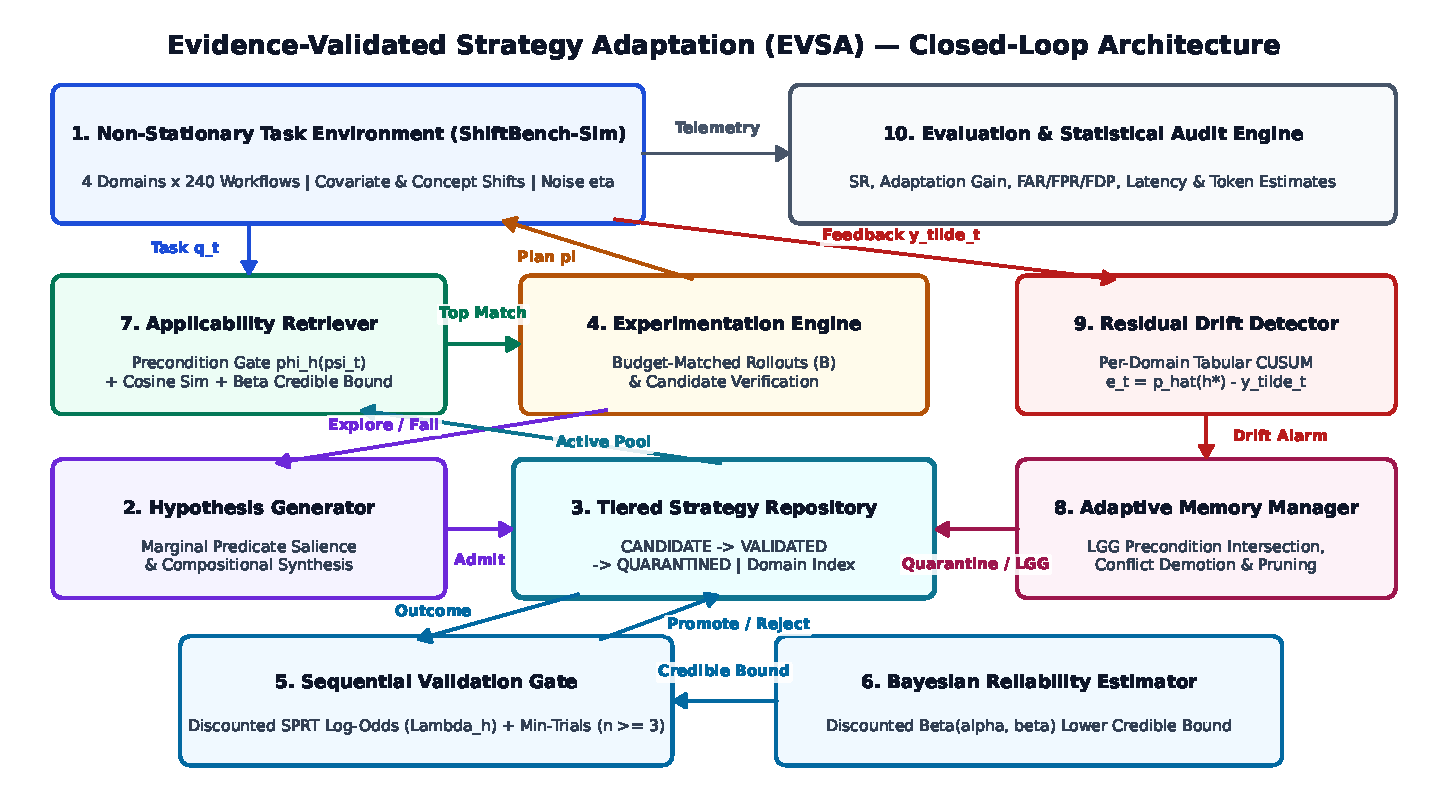
\includegraphics[width=0.96\textwidth]{../figures/fig01_system_architecture.pdf}
  \caption{\textbf{EVSA Ten-Module Closed-Loop System Architecture.} Tasks $q_t$ are matched against precondition- and reliability-gated strategies (Module 7), executed or verified within rollout budget $B$ (Module 4), audited sequentially via discounted SPRT log-odds and Beta lower credible bounds (Modules 5--6), generalized conservatively via Safe LGG (Module 8), and monitored online per domain by a residual tabular CUSUM drift detector (Module 9).}
  \label{fig:arch}
\end{figure*}

\begin{figure*}[t]
  \centering
  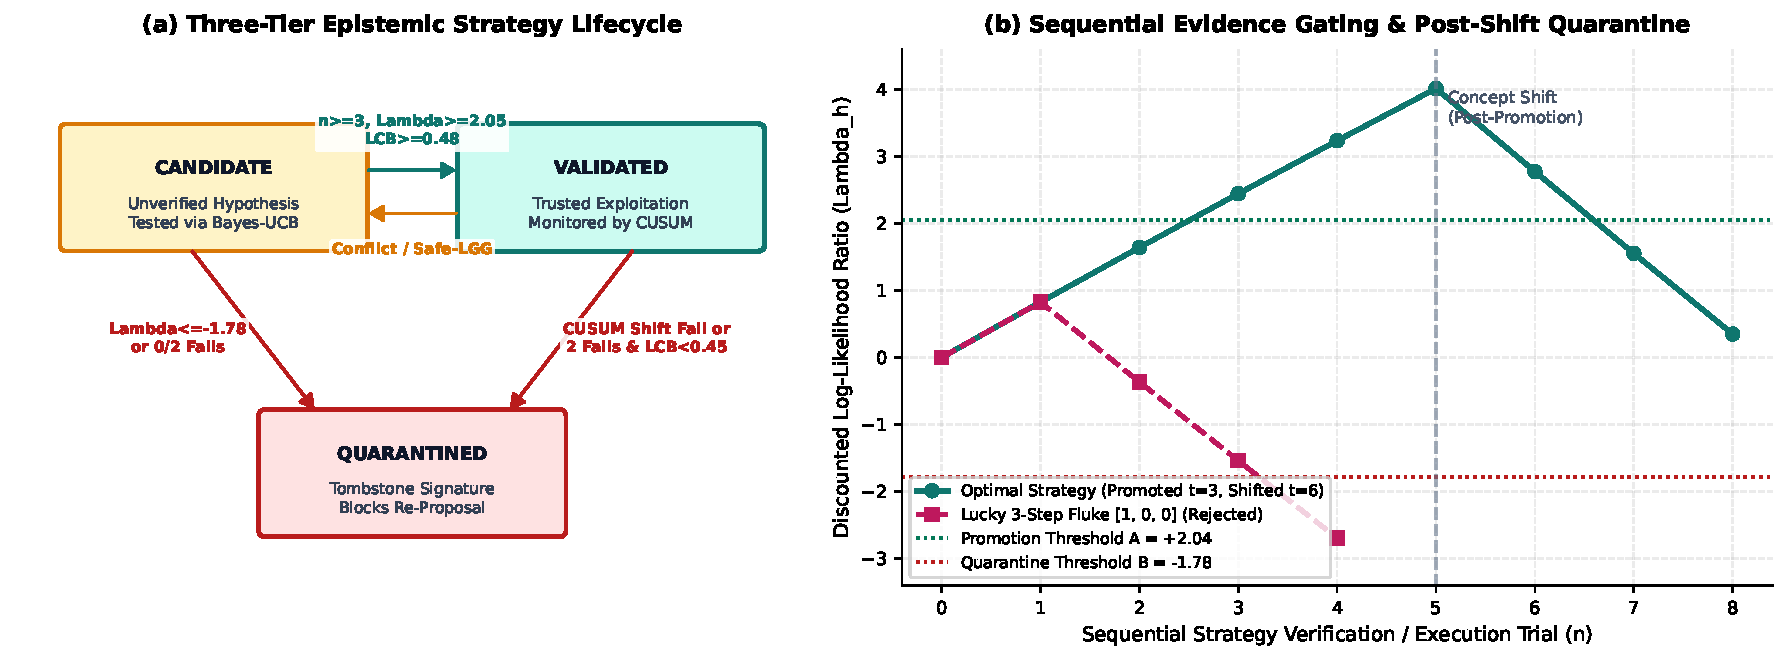
\includegraphics[width=0.96\textwidth]{../figures/fig02_validation_workflow.pdf}
  \caption{\textbf{Strategy Validation Lifecycle and Sequential Evidence Trajectories.} (a) State transitions across \texttt{CANDIDATE}, \texttt{VALIDATED}, and \texttt{QUARANTINED} tiers, including conflict/Safe-LGG demotion and tombstone re-admission blocking. (b) Exact deterministic trajectories of the discounted log-likelihood ratio $\Lambda_h$ ($\gamma=0.985$) showing promotion of a true optimal workflow at $n=3$, rejection of a 1-success lucky fluke $[1,0,0]$, and rapid post-shift decay.}
  \label{fig:val_workflow}
\end{figure*}

\paragraph{Operational Episode Loop.}
Algorithm~\ref{alg:evsa} details EVSA's per-episode decision and update cycle (\texttt{src/\allowbreak agents/\allowbreak evsa\_agent.py}):
\begin{enumerate}
  \item \textbf{Exploitation via Validated Retrieval (Modules 3 \& 7):} Given task $q_t = (x_t, d_t, \psi_t)$, the \textbf{Applicability Retriever} filters \texttt{VALIDATED} strategies in domain $d_t$ whose precondition conjunction $\phi_h(\psi_t) = 1$ holds and whose Bayesian lower credible bound satisfies $\underline{p}_h^{\mathrm{cred}}(\delta) \ge \tau_{\mathrm{rel}} = 0.45$ (Figure~\ref{fig:app_retrieval}a). If a match $h^*$ exists, EVSA records the out-of-sample predictive probability $\hat{p}_{\mathrm{pre}} = \alpha_{h^*}/(\alpha_{h^*} + \beta_{h^*})$, executes $\pi_{h^*}$, updates $(\alpha_{h^*}, \beta_{h^*}, \Lambda_{h^*})$ first with observed feedback $\tilde{y}_t$, and then feeds residual $e_t = \hat{p}_{\mathrm{pre}} - \tilde{y}_t$ to the domain-$d_t$ \textbf{Residual CUSUM Detector} (Module 9).
  \item \textbf{Active Candidate Verification During Adaptation Only (Modules 4--6):} During online learning ($\texttt{learn}=\textbf{true}$), if no \texttt{VALIDATED} strategy applies (or if $\tilde{y}_t = 0$ leaves rollout budget remaining), EVSA selects among precondition-compatible \texttt{CANDIDATE} strategies maximizing a Bayes-UCB utility ($0.85\,I_{0.90}^{-1}(\alpha_h, \beta_h) + \allowbreak 0.15\max(0,\cos(x_t, c_h)) + \allowbreak 0.015|\phi_h|$) \cite{kaufmann2012bayesian}. During frozen evaluation ($\texttt{learn}=\textbf{false}$), unvalidated \texttt{CANDIDATE} strategies are strictly excluded from execution.
  \item \textbf{Salience-Guided Exploration \& Safe LGG Admission (Modules 2 \& 8):} When budget remains and no strategy is selected, the \textbf{Hypothesis Generator} synthesizes a workflow $\pi_{\mathrm{new}}$ (mutating away from tombstoned plans in $\mathcal{M}_{d_t}$ matching $\psi_t$) using marginal step-predicate outcome contrasts accumulated strictly from observed rollouts. Only if $\tilde{y}_t = 1$ is $\pi_{\mathrm{new}}$ admitted to \texttt{CANDIDATE}—or merged into an existing strategy matching $(d_t, \pi_{\mathrm{new}})$ via Safe LGG precondition intersection.
  \item \textbf{Selective Drift Quarantine \& Capacity Pruning (Modules 8 \& 9):} If domain-$d_t$'s CUSUM statistic crosses $h_{\mathrm{drift}}$ (subject to post-reset warmup and cooldown), EVSA immediately quarantines active strategies in $\mathcal{M}_{d_t}$ exhibiting empirical failure ($f_h^{\mathrm{consec}} \ge 1$) or weakened reliability ($\underline{p}_h^{\mathrm{cred}} < 0.58$), while discounting unfalsified strategies in $\mathcal{M}_{d_t}$ back to \texttt{CANDIDATE} for rapid re-verification and leaving all other domains untouched.
\end{enumerate}

\begin{algorithm}[t]
\small
\caption{EVSA Closed-Loop Decision, Safe-LGG Validation, and Selective Drift Quarantine}
\label{alg:evsa}
\begin{algorithmic}[1]
\Require Task $q_t = (x_t, d_t, \psi_t)$, Strategy Repository $\mathcal{M}$, Budget $B$, Mode $\texttt{learn} \in \{\textbf{true}, \textbf{false}\}$
\State $b \leftarrow 0$, $\text{tried} \leftarrow \emptyset$
\While{$b < B$}
  \State $\mathcal{V}_t \leftarrow \{h \in \mathcal{M}_{d_t} \setminus \text{tried} : \tau_h = \texttt{VALIDATED} \land \phi_h(\psi_t) = 1 \land \underline{p}_h^{\mathrm{cred}}(\delta) \ge \tau_{\mathrm{rel}}\}$
  \State $\mathcal{C}_t \leftarrow \{h \in \mathcal{M}_{d_t} \setminus \text{tried} : \tau_h = \texttt{CANDIDATE} \land \phi_h(\psi_t) = 1\}$
  \If{$\mathcal{V}_t \neq \emptyset$ \textbf{or} ($\texttt{learn}$ \textbf{and} $\mathcal{C}_t \neq \emptyset$)}
    \State Select $h^*$ maximizing $U(h, q_t)$ on $\mathcal{V}_t$ if $\mathcal{V}_t \neq \emptyset$, else maximizing $U_{\mathrm{cand}}(h, q_t)$ on $\mathcal{C}_t$
    \State $\text{used\_val} \leftarrow (\tau_{h^*} = \texttt{VALIDATED})$; \quad $\hat{p}_{\mathrm{pre}} \leftarrow \text{PosteriorMean}(h^*)$; \quad $\text{tried} \leftarrow \text{tried} \cup \{h^*\}$
    \State Execute $\pi_{h^*}$, observe $\tilde{y}_t \in \{0,1\}$; \quad $b \leftarrow b + 1$
    \If{$\texttt{learn}$}
      \State Update $(n_{h^*}, \alpha_{h^*}, \beta_{h^*}, f_{h^*}^{\mathrm{consec}}, \Lambda_{h^*}, \tau_{h^*})$ via Eqs.~\eqref{eq:beta_update}--\eqref{eq:tier_rules}
      \If{$\text{used\_val}$ \textbf{and} $\text{UpdateDomainCUSUM}(d_t, \hat{p}_{\mathrm{pre}} - \tilde{y}_t, t) = \texttt{ALARM}$}
        \State Quarantine $h \in \mathcal{M}_{d_t}$ with $f_h^{\mathrm{consec}} \ge 1 \lor \underline{p}_h^{\mathrm{cred}} < 0.58$; discount unfalsified $h \in \mathcal{M}_{d_t}$ to \texttt{CANDIDATE}
      \EndIf
    \EndIf
  \Else
    \State Synthesize non-quarantined plan $\pi_{\mathrm{exp}}$ via observed step-predicate salience; execute $\pi_{\mathrm{exp}}$, observe $\tilde{y}_t$; $b \leftarrow b + 1$
    \If{$\texttt{learn}$ \textbf{and} $\tilde{y}_t = 1$}
      \State Merge via Safe LGG (Eq.~\eqref{eq:lgg}) if compatible peer $h \in \mathcal{M}_{d_t}$ shares $\pi_{\mathrm{exp}}$; else admit new \texttt{CANDIDATE}
    \EndIf
  \EndIf
  \If{$\tilde{y}_t = 1$} \textbf{break} \EndIf
\EndWhile
\end{algorithmic}
\end{algorithm}

% ---------------------------------------------------------------------------
% 9. MATHEMATICAL FORMULATION
% ---------------------------------------------------------------------------
\section{Mathematical Formulation}
\label{sec:math}

\subsection{Discounted Bayesian Beta Posterior and Lower Credible Bounds}
Let $\theta_h \in (0,1)$ denote the unknown conditional success rate of strategy $h$ on tasks satisfying $\phi_h(\psi_t) = 1$ under the active feedback channel. Placing a uniform prior $\theta_h \sim \mathrm{Beta}(\alpha_0, \beta_0)$ ($\alpha_0 = \beta_0 = 1$), we incorporate exponential forgetting factor $\gamma = 0.985$ upon observing outcome $\tilde{y}_n \in \{0,1\}$ (\texttt{src/validation/confidence.py}):
\begin{equation}
  \alpha_h^{(n)} = \alpha_0 + \gamma \bigl(\alpha_h^{(n-1)} - \alpha_0\bigr) + \tilde{y}_n, \qquad
  \beta_h^{(n)}  = \beta_0  + \gamma \bigl(\beta_h^{(n-1)}  - \beta_0\bigr)  + (1 - \tilde{y}_n).
  \label{eq:beta_update}
\end{equation}
The posterior predictive mean is $\hat{p}_h = \alpha_h^{(n)} / (\alpha_h^{(n)} + \beta_h^{(n)})$, and the conservative reliability score is the exact $\delta$-quantile ($\delta = 0.10$) of $\mathrm{Beta}(\alpha_h^{(n)}, \beta_h^{(n)})$ via the inverse regularized incomplete beta function $I_\delta^{-1}$ (with symmetric upper quantile $\bar{p}_h^{\mathrm{cred}} = I_{1-\delta}^{-1}$ for Bayes-UCB candidate exploration):
\begin{equation}
  \underline{p}_h^{\mathrm{cred}}(\delta) = I_{\delta}^{-1}\!\bigl(\alpha_h^{(n)}, \beta_h^{(n)}\bigr), \qquad \text{satisfying } \int_0^{\underline{p}_h^{\mathrm{cred}}(\delta)} \frac{u^{\alpha_h^{(n)}-1}(1-u)^{\beta_h^{(n)}-1}}{\mathrm{B}(\alpha_h^{(n)}, \beta_h^{(n)})}\,du = \delta.
  \label{eq:credible_bound}
\end{equation}
\textbf{Credible Bounds vs.\ Unregularized Empirical Ablation:} Crucially, $\underline{p}_h^{\mathrm{cred}}(\delta)$ is a \emph{discounted Bayesian $(1-\delta)$ lower credible bound}, distinct from a frequentist Clopper-Pearson confidence bound or time-uniform confidence sequence \cite{howard2021time}. Under small sample sizes, $\underline{p}_h^{\mathrm{cred}}(0.10)$ regularizes 1-for-1 flukes ($\alpha=2,\beta=1 \Rightarrow 0.316 < 0.48$) while $\bar{p}_h^{\mathrm{cred}}(0.90)$ protects promising candidates against single stochastic misses. In our \texttt{w/o Confidence Estimation} ablation, Bayesian credible bounds are replaced by the unregularized discounted empirical frequency $\hat{p}_h^{\mathrm{emp}} = (\alpha_h - \alpha_0)/(\alpha_h - \alpha_0 + \beta_h - \beta_0)$ ($0.50$ at $n_h=0$).

\subsection{Discounted Log-Odds Sequential Heuristic (Motivated by Wald's SPRT)}
To separate aligned strategies ($\theta_h \ge p_1$) from suboptimal partial plans ($\theta_h \le p_0$), we specify indifference boundaries $p_0 = 0.35$ and $p_1 = 0.80$ with nominal calibration parameters $(\alpha_{\mathrm{FA}}, \beta_{\mathrm{FR}}) = (0.11, 0.15)$ (\texttt{src/validation/sprt\_validator.py}), yielding log-odds thresholds:
\begin{equation}
  A = \ln\!\left(\frac{1 - \beta_{\mathrm{FR}}}{\alpha_{\mathrm{FA}}}\right) \approx +2.045, \qquad
  B_{\mathrm{low}} = \ln\!\left(\frac{\beta_{\mathrm{FR}}}{1 - \alpha_{\mathrm{FA}}}\right) \approx -1.780.
  \label{eq:sprt_bounds}
\end{equation}
Upon each trial $\tilde{y}_n \in \{0,1\}$, EVSA updates a discounted, clipped log-likelihood ratio $\Lambda_h^{(n)} \in [-\Lambda_{\max}, +\Lambda_{\max}]$ ($\Lambda_{\max} = 6.0$):
\begin{equation}
  \Lambda_h^{(n)} = \mathrm{clip}\!\left(\gamma \Lambda_h^{(n-1)} + \tilde{y}_n \ln\!\left(\frac{p_1}{p_0}\right) + (1 - \tilde{y}_n) \ln\!\left(\frac{1 - p_1}{1 - p_0}\right),\; -\Lambda_{\max},\; +\Lambda_{\max}\right),
  \label{eq:sprt_update}
\end{equation}
where $\ln(p_1/p_0) \approx +0.827$ and $\ln((1-p_1)/(1-p_0)) \approx -1.179$. Tier transitions follow the conjunctive decision rule:
\begin{equation}
  \tau_h^{(n)} =
  \begin{cases}
    \texttt{VALIDATED}, & \text{if } \tau_h^{(n-1)} = \texttt{CANDIDATE} \land n_h \ge n_{\min} \land \Lambda_h^{(n)} \ge A \land \underline{p}_h^{\mathrm{cred}}(0.10) \ge 0.48, \\
    \texttt{QUARANTINED}, & \text{if } \Lambda_h^{(n)} \le B_{\mathrm{low}} \;\lor\; (\tau_h^{(n-1)}=\texttt{CANDIDATE} \land n_h \ge 2 \land s_h = 0) \\
                          & \quad \lor\; (\tau_h^{(n-1)}=\texttt{VALIDATED} \land f_h^{\mathrm{consec}} \ge 2 \land \underline{p}_h^{\mathrm{cred}}(0.10) < 0.45), \\
    \tau_h^{(n-1)}, & \text{otherwise},
  \end{cases}
  \label{eq:tier_rules}
\end{equation}
with $n_{\min} = 3$, cumulative successes $s_h$, and consecutive failures $f_h^{\mathrm{consec}}$. Three consecutive successes produce $\Lambda_h^{(3)} \approx 2.443 \ge 2.045$, promoting $h$ cleanly.

\textbf{Theoretical Audit of Classical SPRT Assumptions:} Classical Wald (1945) guarantees ($\Pr(\text{Accept } H_1 \mid H_0) \le \alpha_{\mathrm{FA}}$) require undiscounted ($\gamma=1$), unclipped i.i.d.\ sampling independent of arm selection \cite{wald1945sequential}. Because Eq.~\eqref{eq:sprt_update} introduces exponential discounting ($\gamma < 1$), clipping ($\pm \Lambda_{\max}$), a hard sample-size floor ($n_{\min}=3$), a joint Beta credible gate, and adaptive Bayes-UCB candidate selection, \emph{classical Wald Type-I/II error bounds do not hold analytically}. We therefore characterize Eqs.~\eqref{eq:sprt_bounds}--\eqref{eq:tier_rules} strictly as an empirically calibrated sequential heuristic and measure its realized candidate-level false-promotion rate directly in Experiment 4 ($8.08\%\text{--}11.32\%$ across $\eta \in [0.10, 0.35]$). Achieving exact finite-sample error guarantees under adaptive bandit stopping requires non-negative test supermartingales / $e$-processes \cite{ramdas2023game}.

\subsection{Applicability-Gated Retrieval and Re-Verified Safe LGG Abstraction}
Each strategy $h$ stores a conjunctive precondition $\phi_h \subseteq \{0,\dots,K-1\} \times \{0,1\}$ evaluated via $\phi_h(\psi_t) = \prod_{(k,v) \in \phi_h} \mathbb{I}[\psi_{t,k} = v] \in \{0,1\}$. When an exploratory workflow $\pi$ succeeds ($\tilde{y}_t = 1$) with induced preconditions $\phi_{\mathrm{new}}$ and matches an active peer $h \in \mathcal{M}_{d_t}$ ($\pi_h = \pi$) differing on $1 \le \Delta \le 2$ shared coordinates, EVSA applies Plotkin's Least General Generalization (LGG) \cite{plotkin1970inductive} (\texttt{src/memory/memory\_manager.py}):
\begin{equation}
  \phi_h^{\mathrm{LGG}} = \bigl\{(k, v) \in \phi_h \cap \phi_{\mathrm{new}}\bigr\}, \qquad \text{subject to } |\phi_h^{\mathrm{LGG}}| \ge K_{\min} = 3.
  \label{eq:lgg}
\end{equation}
\textbf{Safe LGG Re-Verification:} Whenever Eq.~\eqref{eq:lgg} strictly broadens an already-\texttt{VALIDATED} strategy ($|\phi_h^{\mathrm{LGG}}| < |\phi_h|$), preserving \texttt{VALIDATED} status blindly would allow a single noisy false positive ($\tilde{y}_t = 1$) on a neighboring archetype to drop a governing literal and poison future exploitations. EVSA therefore discounts excess pseudo-counts by $\gamma_{\mathrm{LGG}} = 0.80$, clamps $\Lambda_h \leftarrow \min(\gamma_{\mathrm{LGG}}\Lambda_h, A - 0.15)$, and steps $\tau_h$ back to \texttt{CANDIDATE} so that at least one independent confirming trial on the generalized subspace is required before re-promotion.

Retrieval utility enforces both symbolic applicability $\phi_h(\psi_t)=1$ and minimum lower credible reliability $\tau_{\mathrm{rel}} = 0.45$ for \texttt{VALIDATED} strategies ($w_{\mathrm{sem}}=0.28, w_{\mathrm{conf}}=0.52, w_{\mathrm{tier}}=0.20, b_{\mathrm{spec}}=0.015$; \texttt{src/\allowbreak retrieval/\allowbreak retriever.py}):
\begin{equation}
\begin{split}
  U(h, q_t) &= \mathbb{I}[d_h = d_t] \cdot \phi_h(\psi_t) \cdot \mathbb{I}\!\bigl[\underline{p}_h^{\mathrm{cred}}(0.10) \ge \tau_{\mathrm{rel}}\bigr] \\
            &\quad \cdot \Bigl(w_{\mathrm{sem}} \max(0, \cos(x_t, c_h)) + w_{\mathrm{conf}} \underline{p}_h^{\mathrm{cred}}(0.10) + w_{\mathrm{tier}} + b_{\mathrm{spec}}|\phi_h|\Bigr).
\end{split}
  \label{eq:retrieval_utility}
\end{equation}

\begin{figure*}[t]
  \centering
  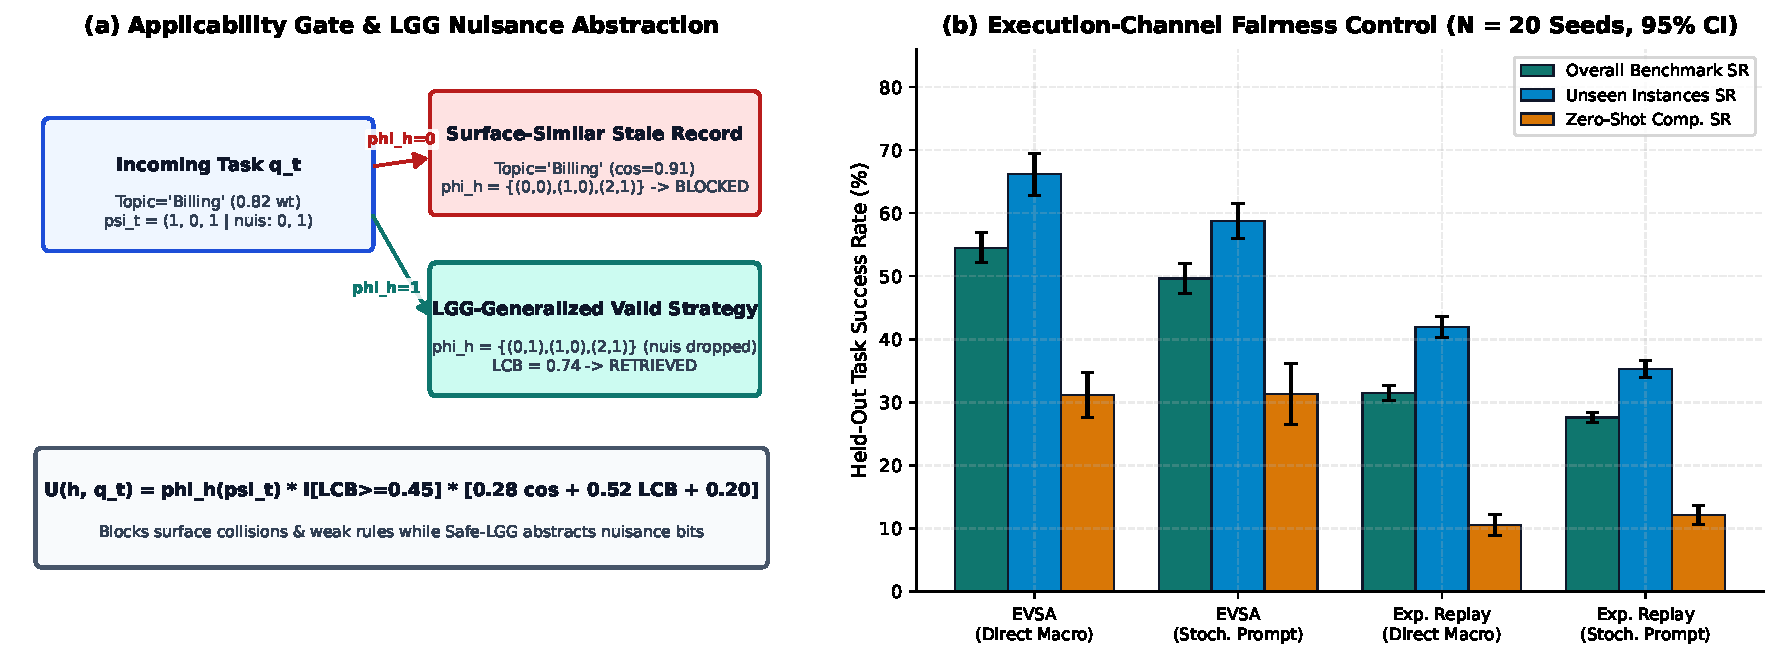
\includegraphics[width=0.96\textwidth]{../figures/fig03_applicability_retrieval.pdf}
  \caption{\textbf{Applicability-Gated Retrieval and Execution-Channel Fairness Parity.} (a) Multiplicative gating $\phi_h(\psi_t)\cdot\mathbb{I}[\underline{p}_h^{\mathrm{cred}} \ge 0.45]$ blocks surface-similar stale records ($\cos=0.91$) while retrieving Safe-LGG generalized valid strategies. (b) Controlled $N=20$ seed fairness experiment decoupling memory-selection quality from execution-channel determinism (\texttt{Direct Macro} vs.\ \texttt{Stochastic Prompt}).}
  \label{fig:app_retrieval}
\end{figure*}

\subsection{Per-Domain Residual Tabular CUSUM Drift Detection}
Let $e_t = \hat{p}_{h^*}^{(t-1)} - \tilde{y}_t \in [-1, 1]$ denote the one-step out-of-sample prediction residual computed \emph{prior} to updating $h^*$ whenever a \texttt{VALIDATED} strategy $h^*$ is executed in domain $d = d_t$ (\texttt{src/drift\_detection/cusum\_detector.py}). EVSA maintains an independent one-sided tabular CUSUM statistic \cite{page1954continuous} per domain $d \in \mathcal{D}$:
\begin{equation}
  S_d^{(t)} = \max\!\bigl(0,\; S_d^{(t-1)} + e_t - \nu_{\mathrm{drift}}\bigr), \qquad S_d^{(0)} = 0,
  \label{eq:cusum}
\end{equation}
with slack $\nu_{\mathrm{drift}} = 0.12$, alarm threshold $h_{\mathrm{drift}} = 1.45$, post-reset observation warmup $n_{\min,\mathrm{obs}} = 3$, and per-domain cooldown of $12$ episodes. Firing $S_d^{(t)} \ge h_{\mathrm{drift}}$ immediately quarantines strategies in $\mathcal{M}_d$ exhibiting $f_h^{\mathrm{consec}} \ge 1$ or $\underline{p}_h^{\mathrm{cred}}(0.10) < 0.58$, discounts unfalsified strategies in $\mathcal{M}_d$ by $\gamma_{\mathrm{shift}} = 0.35$ to \texttt{CANDIDATE}, and resets $S_d^{(t)} \leftarrow 0$ (Figure~\ref{fig:drift}).

\begin{figure*}[t]
  \centering
  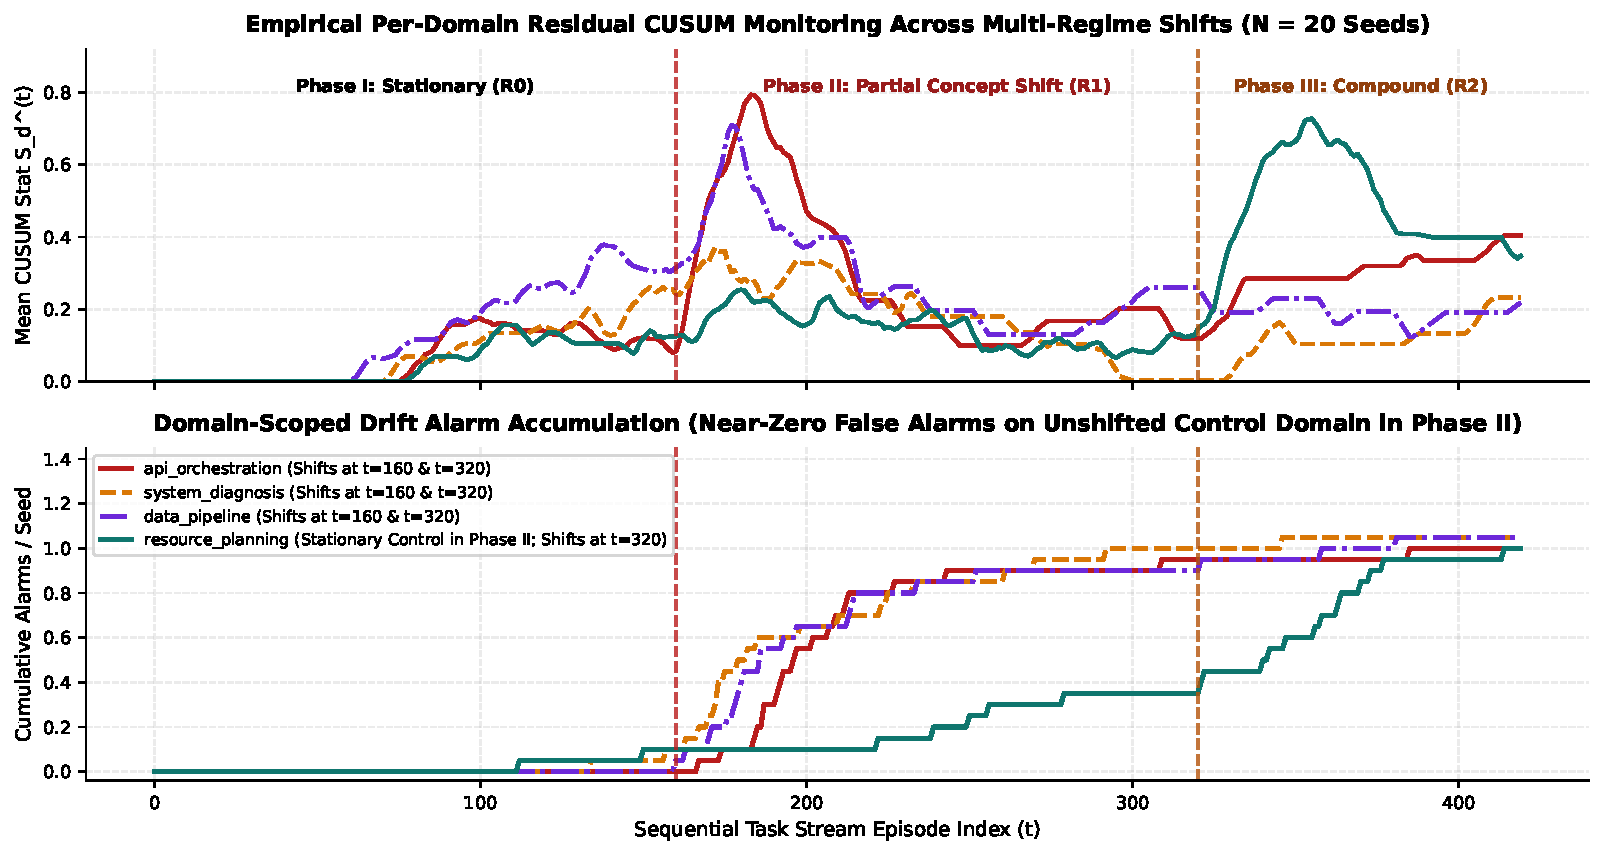
\includegraphics[width=0.96\textwidth]{../figures/fig04_drift_detection.pdf}
  \caption{\textbf{Empirical Per-Domain Residual CUSUM Monitoring Across Multi-Regime Shifts ($N=20$ Seeds).} Top: 5-episode smoothed mean CUSUM statistic $S_d^{(t)}$ across 420 episodes in Experiment 3. Bottom: Cumulative drift alarms per seed. At $t=160$, the three shifted domains spike and trigger quarantine within a mean delay of $38.40$ global episodes ($\approx 9.6$ domain episodes), whereas the stationary control domain (\texttt{resource\_planning}) averages only $0.25$ false alarms across Phase II before genuinely shifting at $t=320$.}
  \label{fig:drift}
\end{figure*}

% ---------------------------------------------------------------------------
% 10. BENCHMARK DESIGN
% ---------------------------------------------------------------------------
\section{Benchmark Design: ShiftBench-Sim v1.0}
Evaluating memory validation, drift invalidation, and noisy-feedback calibration across hundreds of thousands of rollouts requires exact control over ground-truth structural invariants without hidden pretraining leakage. We construct \textbf{ShiftBench-Sim v1.0} (\texttt{src/benchmark/environment.py}), a deterministic symbolic-procedural multi-domain benchmark parameterized as follows:
\begin{itemize}
  \item \textbf{Domains and Heterogeneous Action Space:} $|\mathcal{D}| = 4$ operational domains (\texttt{api\_orchestration}, \texttt{system\_diagnosis}, \texttt{data\_pipeline}, \texttt{resource\_planning}). Each task requires planning an $H=4$-step workflow $\pi \in \mathcal{A}_0 \times \mathcal{A}_1 \times \mathcal{A}_2 \times \mathcal{A}_3$ with action cardinalities $(4, 5, 4, 3)$ ($240$ distinct workflows per domain).
  \item \textbf{Governing vs.\ Nuisance Preconditions:} Each task exposes $K=5$ binary predicates $\psi_t \in \{0,1\}^5$. Bits $(\psi_0, \psi_1, \psi_2)$ define $C = 2^3 = 8$ latent workflow archetypes $c = 4\psi_0 + 2\psi_1 + \psi_2 \in \{0,\dots,7\}$. Bits $(\psi_3, \psi_4)$ are pure nuisance attributes that alter surface context without changing $\pi^*$. Archetypes $c \in \{0,\dots,6\}$ appear during stationary training; \textbf{archetype $c=7$ ($\psi_0=\psi_1=\psi_2=1$) is held out strictly for zero-shot compositional testing}, with Steps 0--2 governed additively by individual bits and Step 3 governed by a non-linear XOR parity interaction ($\psi_0 \oplus \psi_1$).
  \item \textbf{Controlled Surface-Embedding Collisions:} Normalized task embeddings $x_t \in \mathbb{R}^{20}$ ($\|x_t\|_2=1$) concatenate domain features (weight $0.50$), noisy structural features (weight $0.36$), and 8 shared surface-topic vectors (weight $0.82$). Tasks sharing surface topics across conflicting archetypes therefore exhibit high cosine similarity, penalizing precondition-blind retrieval.
  \item \textbf{Regime Shifts and Stochastic Outcome Probabilities:} Regime $r=0$ defines baseline optimal workflows $\pi^*_{d,c,0}$. Regime $r=1$ (abrupt partial-domain concept shift) shifts Steps 1 and 2 by $+2 \pmod{|\mathcal{A}_s|}$ across three domains while keeping \texttt{resource\_planning} invariant ($r=0$) as an unshifted control. Regime $r=2$ (compound shift) shifts Step 0 and Step 2 across all four domains alongside covariate concentration onto $c \in \{4,5,6,7\}$. Executing 4, 3, 2, or $\le 1$ matching steps succeeds with probabilities $(p_{\mathrm{opt}}, p_{\mathrm{sub3}}, p_{\mathrm{sub2}}, p_{\mathrm{sub1}}) = (0.92, 0.28, 0.09, 0.02)$.
  \item \textbf{Strict Zero-Oracle Isolation:} \texttt{TaskInstance} exposes solely observable task inputs and \texttt{RolloutResult} exposes solely observed feedback $(\pi, \tilde{y}_t, \tilde{r}_t, \text{failed\_step})$. Furthermore, \texttt{CalibratedSymbolicLLMBackbone} (\texttt{src/benchmark/llm\_backbone.py}) computes zero-shot step priors ($0.67$ marginal step competence) strictly from observable $(d_t, \psi_t)$ using a linear inclusive-OR heuristic ($\psi_0 \lor \psi_1$) on Step 3—possessing zero access to $\pi^*$, $c(q_t)$, $r(t)$, or the latent XOR rule, as verified by unit tests \texttt{test\_task\_\allowbreak and\_\allowbreak rollout\_\allowbreak have\_\allowbreak zero\_\allowbreak oracle\_\allowbreak fields} and \texttt{test\_zero\_\allowbreak oracle\_\allowbreak leakage\_\allowbreak across\_\allowbreak all\_\allowbreak agent\_\allowbreak and\_\allowbreak backbone\_\allowbreak modules}.
\end{itemize}

% ---------------------------------------------------------------------------
% 11. EXPERIMENTAL METHODOLOGY
% ---------------------------------------------------------------------------
\section{Experimental Methodology}
All agents share the identical \texttt{CalibratedSymbolicLLMBackbone}, identical task streams per seed, and identical per-episode rollout budget $B$ ($B=2$ during adaptation, $B=1$ during frozen evaluation). Six core experiments plus two sensitivity audits are executed across $N=20$ primary seeds ($\{1001, \dots, 1020\}$; extended to $N=30$ seeds $\{1001, \dots, 1030\}$ for stability verification):
\begin{enumerate}
  \item \textbf{Experiment 1 (Unseen Task Generalization):} Online adaptation on $240$ stationary tasks ($r=0, \eta=0, B=2$, archetypes $0\dots 6$), followed by frozen evaluation ($\texttt{learn}=\textbf{false}, B=1$) on $240$ unseen tasks ($160$ unseen surface instances of $c \in \{0\dots 6\}$ and $80$ zero-shot compositional tasks from held-out $c=7$).
  \item \textbf{Experiment 2 (Continual Learning Without Resets):} $320$ sequential training episodes divided into 8 blocks of 40 tasks ($r=0, \eta=0, B=2$), probed ($B=1$) after every block (plus $t=0$) on an independent 96-task held-out suite.
  \item \textbf{Experiment 3 (Multi-Regime Distribution Shift):} $420$-episode continuous stream ($B=2, \eta=0$): Phase I ($t \in [0,160)$, stationary $r=0$), Phase II ($t \in [160,320)$, abrupt concept shift $r=1$ in 3 domains while \texttt{resource\_planning} remains stationary), and Phase III ($t \in [320,420)$, compound shift $r=2$ across all 4 domains over $c \in \{4,5,6,7\}$).
  \item \textbf{Experiment 4 (Misleading \& Noisy Feedback Robustness):} Across symmetric corruption rates $\eta \in \{0.10, 0.25, 0.35\}$, agents train for $200$ noisy episodes followed by $100$ clean episodes ($\eta=0$) to measure Rollout FAR, Candidate FPR, FRR, Active Validated Contamination (FDP), and Clean Recovery SR.
  \item \textbf{Experiment 5 (Leave-One-Out Component Ablation):} Evaluates Full EVSA against five single-module ablations on a $360$-episode stream combining pre-shift noisy feedback ($\eta=0.15, t \in [0,180)$) with an abrupt 3-domain concept shift ($r=1, \eta=0, t \in [180,360)$) plus a 96-task unseen Regime-1 evaluation suite.
  \item \textbf{Experiment 6 (Computational Efficiency \& Projected Token Cost):} Records local wall-clock CPU latency (\texttt{time.perf\_counter}), memory footprint (\texttt{KB}), environment rollouts, and analytically projected token/API costs (modeled at $\$2.50 / \$10.00$ per $10^6$ input/output tokens; $\$0.00$ actual commercial API spend).
\end{enumerate}

% ---------------------------------------------------------------------------
% 12. BASELINE IMPLEMENTATIONS
% ---------------------------------------------------------------------------
\section{Baseline Implementations and Fairness Audit}
\label{sec:baselines}
To ensure budget-matched algorithmic comparisons on ShiftBench-Sim v1.0, we implement four symbolic-procedural baseline adaptations in \texttt{src/agents/baselines.py}—explicitly distinguishing these controlled benchmark adaptations from exact natural-language reproductions of live LLM systems:
\begin{itemize}
  \item \textbf{Baseline A: Static Agent} (\emph{ReAct-style memoryless adaptation} \cite{yao2023react}): Zero cross-episode memory; samples workflows strictly from \texttt{CalibratedSymbolicLLMBackbone} within rollout budget $B$.
  \item \textbf{Baseline B: Conventional Memory Agent} (\emph{Generative-Agents-style episodic buffer} \cite{park2023generative}): Stores up to $400$ episodic records scored by $0.55\cos(x_t, x_i) + 0.20\cdot 0.993^{\Delta t} + 0.25\,\tilde{r}_i$, conditioning generation on top-$3$ positive matches (weighted adherence $\in [0.55, 0.96]$).
  \item \textbf{Baseline C: Reflection Agent} (\emph{Reflexion-style sliding critique adaptation} \cite{shinn2023reflexion}): Maintains per-domain sliding buffers ($10$/domain) of step-failure avoidance constraints and successful workflows without multi-trial statistical gating or drift quarantine.
  \item \textbf{Baseline D: Experience Replay Agent} (\emph{CER/AWM-style distilled workflow buffer} \cite{liu2025cer,wang2025awm}): Retains successful ($\tilde{y}_t=1$) workflows ($200$ max, centroid-deduplicated at $\cos > 0.80$), retrieving top-$3$ domain matches above $\cos > 0.25$.
\end{itemize}

\paragraph{Audit of Execution-Channel Asymmetry and Controlled Parity Design.}
In default mode, once a strategy reaches \texttt{VALIDATED}, EVSA invokes $\pi_h$ directly as a compiled deterministic macro, whereas Baselines B--D pass retrieved workflows through \texttt{backbone.generate\_plan} (weighted adherence $\le 0.96$). To prevent misattributing macro determinism to memory quality, we evaluate a full $2 \times 2$ execution-channel parity control (\texttt{Direct Macro} vs.\ \texttt{Stochastic Prompt} in both EVSA and Experience Replay) across $N=20$ seeds (Figure~\ref{fig:app_retrieval}b and Table~\ref{tab:fairness}).

% ---------------------------------------------------------------------------
% 13. EXPERIMENTAL RESULTS
% ---------------------------------------------------------------------------
\section{Experimental Results}
\label{sec:results}

\subsection{Experiment 1: Unseen Task Generalization and Execution Parity}
Table~\ref{tab:exp1} and Figure~\ref{fig:exp1} present held-out generalization across $N=20$ seeds ($240$ unseen tasks/seed, executing strictly \texttt{VALIDATED} strategies during frozen evaluation). EVSA achieves \textbf{54.50\% $\pm$ 5.04\%} overall task success (95\% CI $[52.14\%, 56.86\%]$, median $53.75\%$, exact plan accuracy $45.40\%$), outperforming \emph{Static} ($26.48\%$, $+105.82\%$ relative, $d_z = 4.51$), \emph{Conventional Memory} ($29.62\%$, $+83.97\%$, $d_z = 4.47$), \emph{Reflection} ($25.65\%$, $+112.51\%$, $d_z = 4.31$), and \emph{Experience Replay} ($27.58\%$, $+97.58\%$, $d_z = 6.35$), with all four Holm-Bonferroni adjusted paired $t$-test $p$-values $\le 8.15 \times 10^{-14}$. Extending Experiment 1 to \textbf{$N=30$ independent seeds} confirms tight distributional stability: EVSA achieves \textbf{55.17\% $\pm$ 5.62\%} (95\% CI $[53.07\%, 57.27\%]$) versus $25.18\%\text{--}29.12\%$ across baselines.

\begin{table*}[t]
\centering
\caption{Experiment 1: Held-out unseen benchmark generalization ($N=20$ seeds, 240 tasks/seed; Mean $\pm$ SD and $[95\%\text{ CI}]$).}
\label{tab:exp1}
\resizebox{\textwidth}{!}{%
\begin{tabular}{lccccc}
\toprule
\textbf{Agent Architecture} & \textbf{Overall SR (\%)} & \textbf{Exact Plan Acc.\ (\%)} & \textbf{Unseen Instances SR (\%)} & \textbf{Zero-Shot Comp.\ $c=7$ (\%)} & \textbf{Avg.\ Reward} \\
\midrule
Baseline A: Static & $26.48 \pm 3.04$ $[25.06, 27.90]$ & $12.38 \pm 2.46$ & $30.75 \pm 3.78$ & $17.94 \pm 4.61$ & $0.386 \pm 0.023$ \\
Baseline B: Conventional Memory & $29.62 \pm 2.77$ $[28.33, 30.92]$ & $19.60 \pm 2.51$ & $37.81 \pm 3.39$ & $13.25 \pm 2.82$ & $0.410 \pm 0.021$ \\
Baseline C: Reflection & $25.65 \pm 3.61$ $[23.96, 27.33]$ & $13.56 \pm 3.23$ & $29.81 \pm 4.08$ & $17.31 \pm 5.88$ & $0.377 \pm 0.030$ \\
Baseline D: Experience Replay & $27.58 \pm 1.74$ $[26.77, 28.40]$ & $15.69 \pm 1.82$ & $35.31 \pm 2.96$ & $12.12 \pm 3.32$ & $0.389 \pm 0.016$ \\
\midrule
\textbf{Proposed Agent E: EVSA} & $\mathbf{54.50 \pm 5.04}$ $\mathbf{[52.14, 56.86]}$ & $\mathbf{45.40 \pm 7.01}$ & $\mathbf{66.19 \pm 7.11}$ & $\mathbf{31.13 \pm 7.67}$ & $\mathbf{0.646 \pm 0.041}$ \\
\bottomrule
\end{tabular}}
\end{table*}

\begin{figure*}[t]
  \centering
  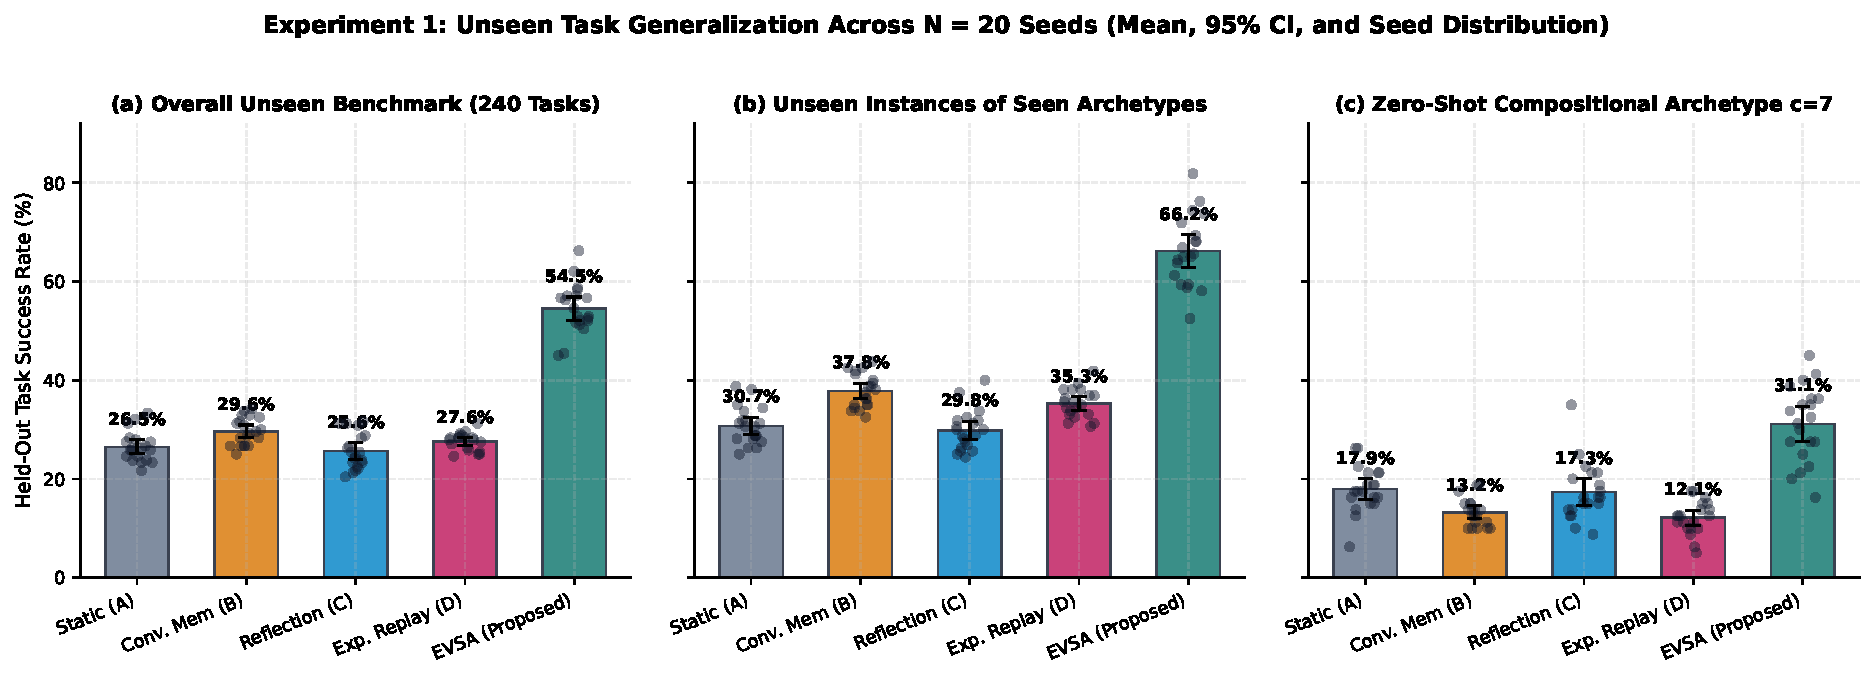
\includegraphics[width=0.96\textwidth]{../figures/fig05_exp1_generalization.pdf}
  \caption{\textbf{Experiment 1 Unseen Generalization Across Splits ($N=20$ Seeds).} Bars depict group means with 95\% CIs; overlaid points show individual seed realizations. Memory baselines suffer negative transfer on zero-shot archetype $c=7$ ($12.1\%\text{--}17.3\%$ vs.\ Static $17.9\%$), whereas EVSA composes validated marginal operators on Steps 0--2 to reach $31.1\%$ on $c=7$ and $66.2\%$ on unseen instances of seen archetypes.}
  \label{fig:exp1}
\end{figure*}

\textbf{Sub-Split Decomposition \& Compositional Parity Ceiling:} On unseen surface instances of seen archetypes ($c \in \{0,\dots,6\}$), Conventional Memory ($37.81\%$) and Experience Replay ($35.31\%$) modestly improve over Static ($30.75\%$), whereas EVSA reaches \textbf{66.19\% $\pm$ 7.11\%} by blocking surface-topic collisions and abstracting nuisance bits $(\psi_3,\psi_4)$. On \textbf{zero-shot compositional archetype $c=7$ ($\psi_0=\psi_1=\psi_2=1$)}—where the non-oracle backbone's linear inclusive-OR heuristic predicts the wrong Step-3 operator—Conventional Memory ($13.25\%$) and Experience Replay ($12.12\%$) drop below Static ($17.94\%$) due to surface collisions with seen archetypes. Because EVSA's precondition gate rejects colliding whole plans while its Hypothesis Generator composes validated step-level marginal operators across Steps 0, 1, and 2 (achieving 3-of-4 step alignment with $p_{\mathrm{sub3}}=0.28$), EVSA reaches \textbf{31.13\% $\pm$ 7.67\%} ($+13.19\text{ pp}$ over Static, $d_z = 1.57, p_{\mathrm{Holm}} = 1.07 \times 10^{-6}$; $+19.00\text{ pp}$ over Replay, $d_z = 2.12, p_{\mathrm{Holm}} = 4.87 \times 10^{-8}$), while remaining honestly bounded well below seen-archetype accuracy ($66.19\%$) because first-order marginal salience cannot deduce the latent Step-3 XOR parity flip zero-shot.

\textbf{Execution-Channel Fairness Control (Table~\ref{tab:fairness}):} Restricting EVSA to execute \texttt{VALIDATED} plans through the exact same stochastic prompt-conditioning channel as Experience Replay yields \textbf{49.62\% $\pm$ 4.98\%}, beating \texttt{Replay (Stochastic Prompt)} ($27.58\%$) by \textbf{$+22.04$ pp} ($d_z = 4.09, p_{\mathrm{Holm}} = 1.57 \times 10^{-13}$). Conversely, granting deterministic macro execution to Experience Replay raises its unseen-instance accuracy ($35.31\% \to 41.97\%$) but \emph{worsens} zero-shot compositional accuracy ($12.12\% \to 10.50\%$) by enforcing 100\% obedience to colliding workflows, yielding $31.48\% \pm 2.45\%$ overall ($-23.02\text{ pp}$ below \texttt{EVSA Direct Macro}, $d_z = 4.47, p_{\mathrm{Holm}} = 6.41 \times 10^{-14}$). Thus $\sim 82\%$ of EVSA's $+26.92\text{ pp}$ total advantage over Experience Replay stems purely from statistical validation and precondition gating, while $\sim 18\%$ ($+4.88\text{ pp}$) comes from deterministic macro compilation once validated.

\begin{table}[t]
\centering
\caption{Execution-Channel Fairness Parity Control on Experiment 1 ($N=20$ seeds).}
\label{tab:fairness}
\small
\begin{tabular}{lccc}
\toprule
\textbf{Controlled Variant} & \textbf{Overall SR (\%)} & \textbf{Unseen Inst.\ (\%)} & \textbf{Zero-Shot Comp.\ (\%)} \\
\midrule
EVSA (\texttt{direct\_macro}) & $\mathbf{54.50 \pm 5.04}$ & $\mathbf{66.19 \pm 7.11}$ & $\mathbf{31.13 \pm 7.67}$ \\
EVSA (\texttt{stochastic\_prompt}) & $49.62 \pm 4.98$ & $58.78 \pm 5.90$ & $31.31 \pm 10.21$ \\
Exp.\ Replay (\texttt{direct\_macro}) & $31.48 \pm 2.45$ & $41.97 \pm 3.64$ & $10.50 \pm 3.59$ \\
Exp.\ Replay (\texttt{stochastic\_prompt}) & $27.58 \pm 1.74$ & $35.31 \pm 2.96$ & $12.12 \pm 3.32$ \\
\bottomrule
\end{tabular}
\end{table}

\subsection{Experiment 2: Continual Learning Without Resets}
Across 320 continual training episodes (Figure~\ref{fig:exp2} and Table~\ref{tab:exp2}), all agents start at $29.27\%$ pre-adaptation accuracy. After Block 1 (40 episodes), Conventional Memory ($24.01\%$), Reflection ($26.51\%$), and Experience Replay ($25.00\%$) dip \emph{below} their zero-shot starting point due to premature exploitation of sparse, colliding exemplars, whereas EVSA rises immediately to \textbf{32.86\%} ($p_{\mathrm{Holm}} \le 9.21 \times 10^{-4}$ vs.\ all four baselines) because unproven hypotheses remain confined to \texttt{CANDIDATE}. By Block 8 ($t=320$), EVSA reaches \textbf{65.21\% $\pm$ 8.52\%} ($+35.94\text{ pp}$ gain, $+126.85\%$ relative; $d_z \in [3.00, 5.42], p_{\mathrm{Holm}} \le 3.85 \times 10^{-11}$ vs.\ all baselines at $27.55\%\text{--}35.68\%$), while retaining only \textbf{21.50} active validated strategies (compared to $143.65$ retained workflows in Experience Replay and $399.4$ episodic records in Conventional Memory). Stationary false CUSUM alarms average just $0.95$ across all 320 episodes.

\begin{table*}[t]
\centering
\caption{Experiment 2: Continual learning trajectory across 320 episodes ($N=20$ seeds).}
\label{tab:exp2}
\resizebox{\textwidth}{!}{%
\begin{tabular}{lcccccc}
\toprule
\textbf{Agent Architecture} & \textbf{Init SR (\%)} & \textbf{Block 1 SR (\%)} & \textbf{Final Block 8 SR (\%)} & \textbf{Abs.\ Gain (pp)} & \textbf{Active Valid/Retained} & \textbf{Rejected/Quarantined} \\
\midrule
Baseline A: Static & $29.27$ & $29.22 \pm 4.10$ & $28.23 \pm 4.10$ & $-1.04$ & $0.00$ & $0.00$ \\
Baseline B: Conventional Memory & $29.27$ & $24.01 \pm 4.48$ & $35.68 \pm 5.47$ & $+6.41$ & $125.15$ & $274.85$ \\
Baseline C: Reflection & $29.27$ & $26.51 \pm 4.41$ & $27.55 \pm 6.25$ & $-1.72$ & $155.15$ & $26.85$ \\
Baseline D: Experience Replay & $29.27$ & $25.00 \pm 4.84$ & $32.29 \pm 4.06$ & $+3.02$ & $143.65$ & $381.80$ \\
\midrule
\textbf{Proposed Agent E: EVSA} & $\mathbf{29.27}$ & $\mathbf{32.86 \pm 3.47}$ & $\mathbf{65.21 \pm 8.52}$ & $\mathbf{+35.94}$ & $\mathbf{21.50}$ & $\mathbf{23.20}$ \\
\bottomrule
\end{tabular}}
\end{table*}

\begin{figure*}[t]
  \centering
  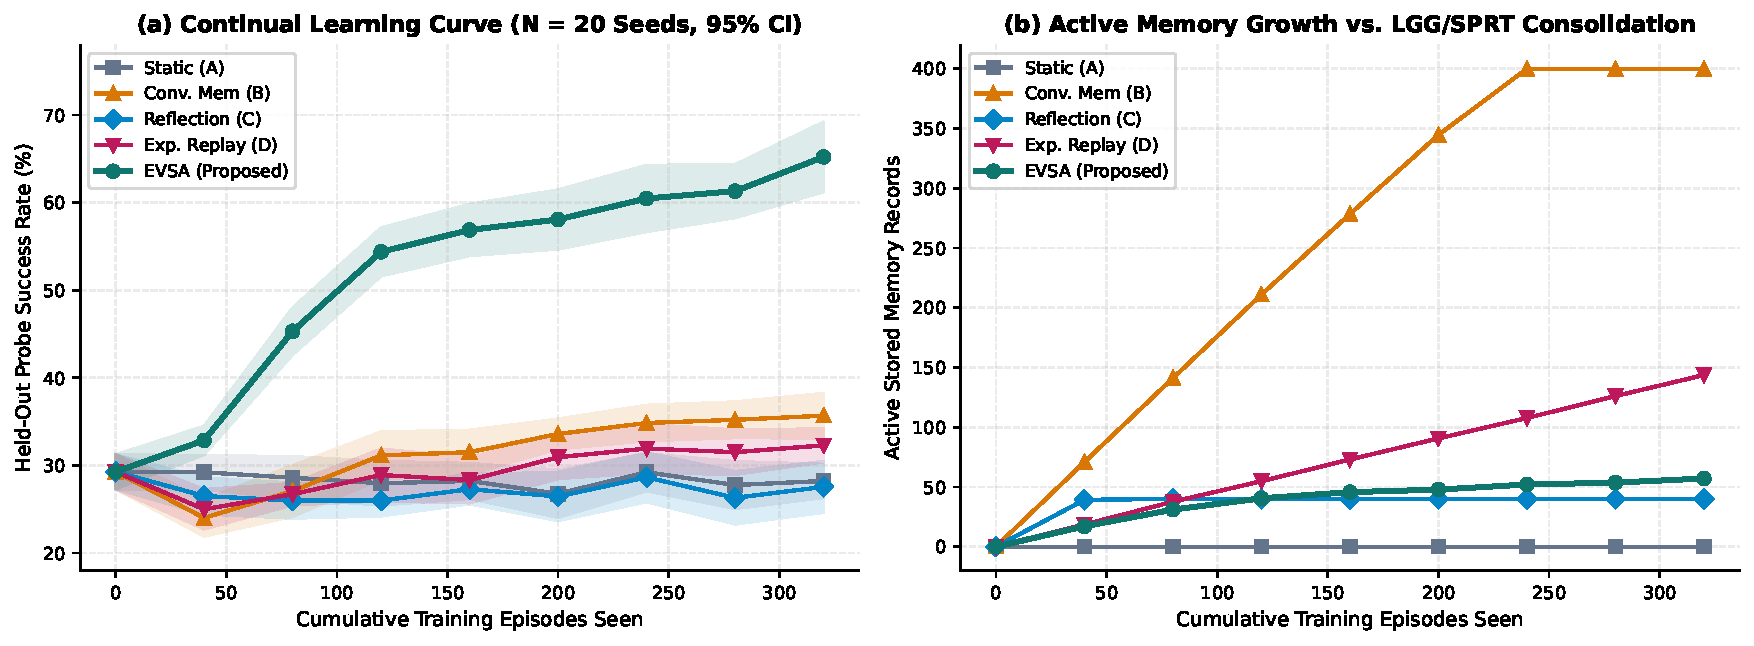
\includegraphics[width=0.96\textwidth]{../figures/fig06_exp2_continual_learning.pdf}
  \caption{\textbf{Experiment 2 Continual Learning and Strategy Consolidation ($N=20$ Seeds).} (a) Held-out probe success rate across 8 blocks (shaded 95\% CIs). (b) Active memory store size showing compact asymptotic convergence in EVSA as Safe LGG merges nuisance variants toward the 28 underlying domain-archetype invariants.}
  \label{fig:exp2}
\end{figure*}

\subsection{Experiment 3: Adaptation Under Multi-Regime Distribution Shift}
Figure~\ref{fig:exp3} and Table~\ref{tab:exp3} track adaptation across Phase I ($t \in [0,160)$, stationary), Phase II ($t \in [160,320)$, 3-domain concept shift), and Phase III ($t \in [320,420)$, 4-domain compound + covariate shift). Prior to $t=160$, EVSA reaches $81.75\%$ streaming success (vs.\ $50.00\%\text{--}54.62\%$). At the abrupt concept shift ($t=160$), EVSA drops transiently to $36.00\%$ shock SR as pre-shift strategies fail, triggering per-domain residual CUSUM alarms within a mean delay of $38.40$ global episodes (Figure~\ref{fig:drift}). Selectively quarantining failed routines and validating Regime-1 replacements lifts EVSA to \textbf{56.80\% $\pm$ 8.76\%} recovered post-shift SR—an \textbf{Adaptation Gain of $+20.80$ pp} versus $-1.90\text{ to }+4.70\text{ pp}$ across baselines ($d_z \in [0.96, 1.36]$, $p_{\mathrm{Holm}} \le 4.08 \times 10^{-4}$), and reaches \textbf{34.88\%} under the Phase III compound shift (vs.\ $9.00\%\text{--}17.00\%$).

\begin{table*}[t]
\centering
\caption{Experiment 3: Multi-regime distribution shift adaptation and selective retention ($N=20$ seeds).}
\label{tab:exp3}
\resizebox{\textwidth}{!}{%
\begin{tabular}{lccccccc}
\toprule
\textbf{Agent Architecture} & \textbf{Pre-Shift SR (\%)} & \textbf{Shock SR (\%)} & \textbf{Recovered SR (\%)} & \textbf{Adapt.\ Gain (pp)} & \textbf{Recov.\ Ratio (\%)} & \textbf{Unshifted Dom.\ (\%)} & \textbf{Phase III SR (\%)} \\
\midrule
Baseline A: Static & $50.00 \pm 8.58$ & $23.20 \pm 6.44$ & $25.40 \pm 6.99$ & $+2.20 \pm 9.06$ & $52.30 \pm 17.25$ & $51.51 \pm 9.11$ & $9.00 \pm 5.40$ \\
Baseline B: Conventional Memory & $54.62 \pm 7.04$ & $28.20 \pm 10.58$ & $32.90 \pm 7.12$ & $+4.70 \pm 12.93$ & $61.03 \pm 14.89$ & $57.49 \pm 8.91$ & $12.50 \pm 5.00$ \\
Baseline C: Reflection & $51.12 \pm 8.56$ & $29.00 \pm 8.60$ & $27.10 \pm 7.15$ & $-1.90 \pm 12.11$ & $53.93 \pm 14.65$ & $51.13 \pm 10.60$ & $17.00 \pm 6.57$ \\
Baseline D: Experience Replay & $54.25 \pm 8.85$ & $27.40 \pm 8.64$ & $30.80 \pm 7.55$ & $+3.40 \pm 10.66$ & $58.55 \pm 19.09$ & $56.40 \pm 9.26$ & $11.88 \pm 6.58$ \\
\midrule
\textbf{Proposed Agent E: EVSA} & $\mathbf{81.75 \pm 6.29}$ & $\mathbf{36.00 \pm 10.46}$ & $\mathbf{56.80 \pm 8.76}$ & $\mathbf{+20.80 \pm 12.49}$ & $\mathbf{70.22 \pm 14.23}$ & $\mathbf{82.21 \pm 11.21}$ & $\mathbf{34.88 \pm 8.90}$ \\
\bottomrule
\end{tabular}}
\end{table*}

\begin{figure*}[t]
  \centering
  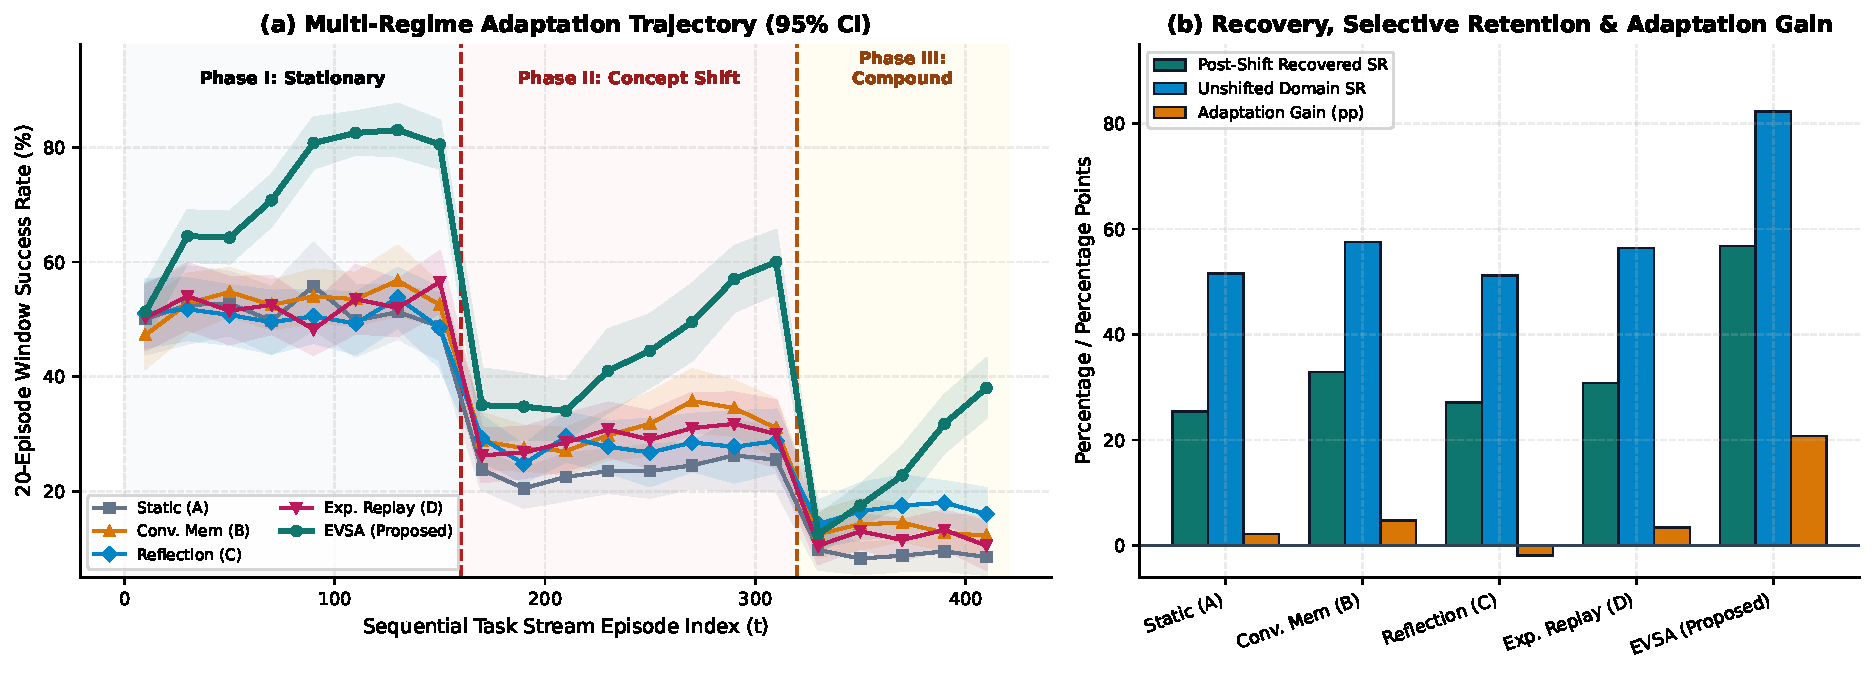
\includegraphics[width=0.96\textwidth]{../figures/fig07_exp3_shift_adaptation.pdf}
  \caption{\textbf{Experiment 3 Multi-Regime Shift Trajectory and Selective Retention ($N=20$ Seeds).} (a) 20-episode sliding window success across Stationary ($t < 160$), Partial Concept Shift ($160 \le t < 320$), and Compound Shift ($t \ge 320$). (b) Recovered post-shift SR ($56.80\%$), unshifted-domain retention ($82.21\%$), and changepoint Adaptation Gain ($+20.80\text{ pp}$).}
  \label{fig:exp3}
\end{figure*}

Simultaneously, on the stationary control domain (\texttt{resource\_planning}), EVSA preserves \textbf{82.21\% $\pm$ 11.21\%} accuracy throughout Phase II ($+24.72\text{ to }+31.07\text{ pp}$ above baselines, $p_{\mathrm{Holm}} \le 4.08 \times 10^{-6}$), confirming zero collateral forgetting. We also report a subtle metric artifact on \emph{proportional Recovery Ratio} ($\mathrm{SR}_{\mathrm{rec}} / \mathrm{SR}_{\mathrm{pre}}$): while EVSA ($70.22\%$) significantly exceeds Static ($52.30\%, p_{\mathrm{Holm}}=0.0017$) and Reflection ($53.93\%, p_{\mathrm{Holm}}=0.0076$), its comparisons versus Conventional Memory ($61.03\%$) and Experience Replay ($58.55\%$) are \textbf{not statistically significant} ($p_{\mathrm{Holm}} = 0.0988$) because those baselines divide stagnant post-shift scores ($\sim 31\%\text{--}33\%$) by much lower pre-shift denominators ($\sim 54\%$ vs.\ EVSA's $81.75\%$).

\subsection{Experiment 4: Feedback Corruption and Safe-LGG Store Decomposition}
Table~\ref{tab:exp4} and Figure~\ref{fig:exp4} evaluate robustness when $\eta \in \{0.10, 0.25, 0.35\}$ of environment outcomes are symmetrically inverted during $t \in [0, 200)$ before clean feedback resumes ($t \in [200, 300)$). Unvalidated memory baselines accept $21.93\%\text{--}38.71\%$ of suboptimal rollouts, poisoning $58.70\%\text{--}85.50\%$ of their active memory and capping post-corruption clean recovery at $45.20\%\text{--}52.30\%$. In contrast, EVSA restricts Rollout FAR to \textbf{1.34\%, 1.76\%, and 2.53\%}, significantly reduces active memory contamination across \textbf{all three noise levels} (including $\eta=0.35$: $68.29\%$ vs.\ $83.12\%\text{--}85.50\%$, $p_{\mathrm{Holm}} = 0.0063$), and recovers rapidly to \textbf{84.10\%, 77.30\%, and 74.90\%} clean accuracy ($d_z \in [2.45, 4.85]$, $p_{\mathrm{Holm}} \le 1.95 \times 10^{-9}$).

\begin{table*}[t]
\centering
\caption{Experiment 4: Misleading feedback calibration, store decomposition, and clean recovery ($N=20$ seeds).}
\label{tab:exp4}
\resizebox{\textwidth}{!}{%
\begin{tabular}{clcccccc}
\toprule
\textbf{Noise $\eta$} & \textbf{Agent Architecture} & \textbf{Rollout FAR (\%)} & \textbf{Cand.\ FPR (\%)} & \textbf{FRR (\%)} & \textbf{Noisy FDP / Contam.\ (\%)} & \textbf{Post-Clean FDP (\%)} & \textbf{Clean Recovery SR (\%)} \\
\midrule
\multirow{4}{*}{$0.10$}
 & Conventional Memory (B) & $21.99 \pm 1.67$ & $21.99 \pm 1.67$ & $16.35 \pm 4.45$ & $58.70 \pm 5.87$ & $52.03 \pm 4.14$ & $51.20 \pm 8.09$ \\
 & Reflection (C)          & $22.44 \pm 2.19$ & $22.44 \pm 2.19$ & $15.52 \pm 5.76$ & $73.08 \pm 10.13$ & $65.82 \pm 13.57$ & $47.50 \pm 7.56$ \\
 & Experience Replay (D)   & $21.93 \pm 1.91$ & $21.93 \pm 1.91$ & $16.65 \pm 5.92$ & $61.27 \pm 6.44$ & $57.50 \pm 6.31$ & $52.30 \pm 9.11$ \\
 & \textbf{EVSA (Proposed)}& $\mathbf{1.34 \pm 0.73}$ & $\mathbf{8.08 \pm 4.03}$ & $44.11 \pm 12.26$ & $\mathbf{35.46 \pm 10.73}$ & $\mathbf{21.79 \pm 6.63}$ & $\mathbf{84.10 \pm 5.64}$ \\
\midrule
\multirow{4}{*}{$0.25$}
 & Conventional Memory (B) & $32.81 \pm 2.05$ & $32.81 \pm 2.05$ & $30.82 \pm 8.69$ & $76.35 \pm 4.71$ & $65.10 \pm 5.41$ & $49.90 \pm 6.50$ \\
 & Reflection (C)          & $32.56 \pm 2.57$ & $32.56 \pm 2.57$ & $30.75 \pm 5.59$ & $82.94 \pm 8.20$ & $65.17 \pm 13.53$ & $48.60 \pm 7.26$ \\
 & Experience Replay (D)   & $31.34 \pm 1.63$ & $31.34 \pm 1.63$ & $31.12 \pm 6.63$ & $77.65 \pm 4.65$ & $70.51 \pm 4.19$ & $47.10 \pm 6.97$ \\
 & \textbf{EVSA (Proposed)}& $\mathbf{1.76 \pm 0.66}$ & $\mathbf{8.64 \pm 3.17}$ & $59.01 \pm 18.01$ & $\mathbf{46.36 \pm 18.44}$ & $\mathbf{24.40 \pm 12.60}$ & $\mathbf{77.30 \pm 10.04}$ \\
\midrule
\multirow{4}{*}{$0.35$}
 & Conventional Memory (B) & $38.71 \pm 2.34$ & $38.71 \pm 2.34$ & $35.53 \pm 8.00$ & $83.12 \pm 3.61$ & $70.75 \pm 4.08$ & $47.60 \pm 8.77$ \\
 & Reflection (C)          & $37.87 \pm 2.05$ & $37.87 \pm 2.05$ & $38.93 \pm 7.50$ & $85.50 \pm 6.98$ & $71.09 \pm 11.94$ & $49.40 \pm 7.92$ \\
 & Experience Replay (D)   & $37.00 \pm 1.98$ & $37.00 \pm 1.98$ & $38.94 \pm 7.31$ & $83.49 \pm 3.66$ & $75.83 \pm 3.28$ & $45.20 \pm 7.66$ \\
 & \textbf{EVSA (Proposed)}& $\mathbf{2.53 \pm 0.98}$ & $\mathbf{11.32 \pm 4.38}$ & $65.44 \pm 16.15$ & $\mathbf{68.29 \pm 19.88}$ & $\mathbf{30.60 \pm 17.14}$ & $\mathbf{74.90 \pm 5.56}$ \\
\bottomrule
\end{tabular}}
\end{table*}

\begin{figure*}[t]
  \centering
  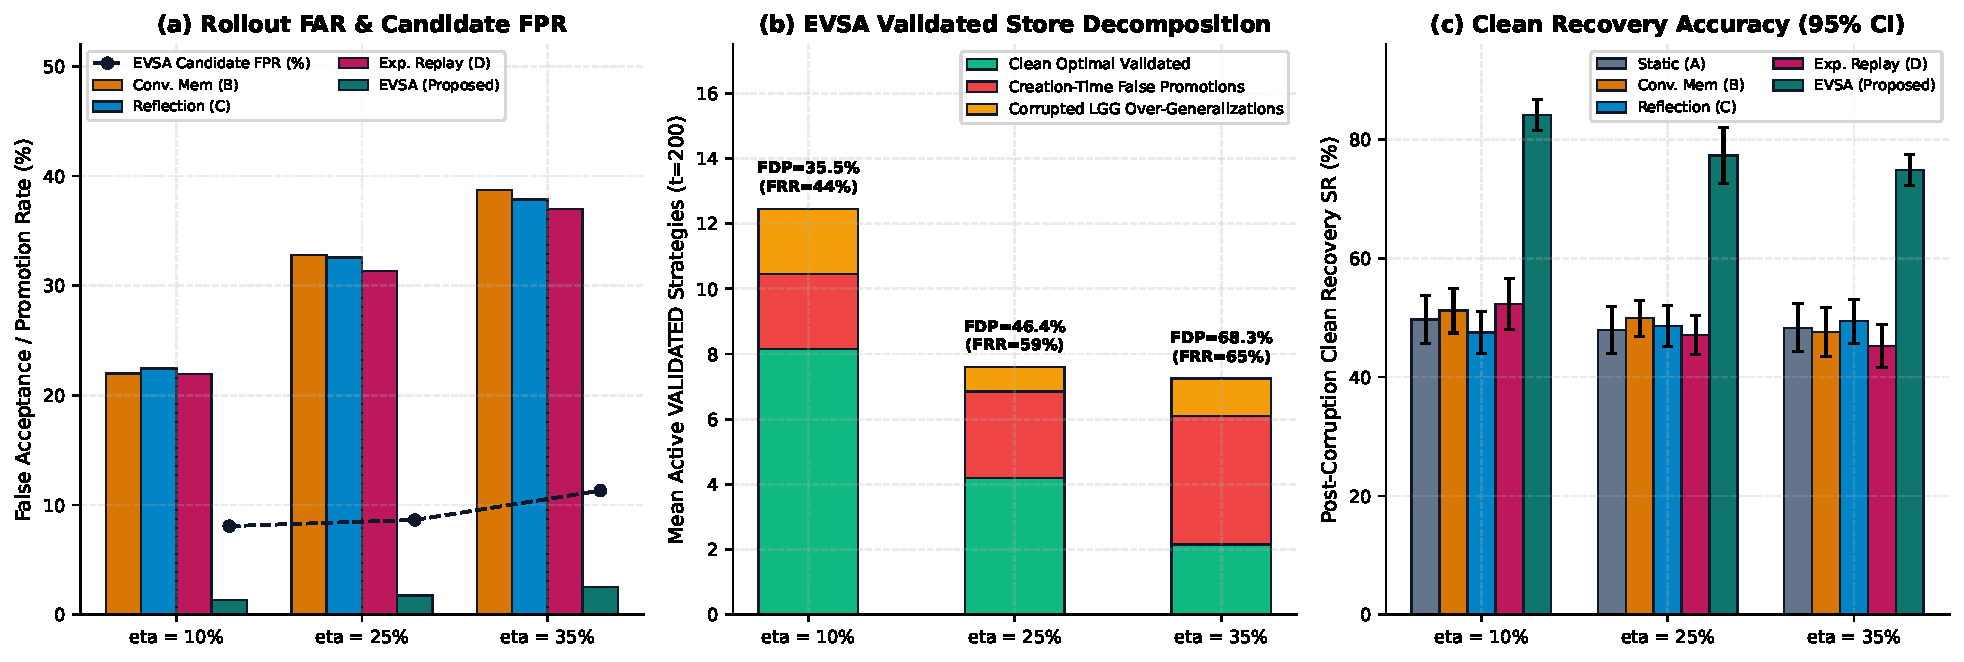
\includegraphics[width=0.96\textwidth]{../figures/fig08_exp4_feedback_corruption.pdf}
  \caption{\textbf{Experiment 4 Feedback Corruption Calibration and Store Decomposition ($N=20$ Seeds).} (a) Rollout FAR vs.\ EVSA Candidate FPR ($\le 11.32\%$). (b) Exact decomposition of active \texttt{VALIDATED} strategies at $t=200$ into Clean Optimal, Creation-Time False Promotions, and Corrupted LGG Over-Generalizations, illustrating how Safe LGG bounds over-generalization to $0.75\text{--}2.00$ rules while high FRR ($65.44\%$ at $\eta=0.35$) shrinks the clean denominator ($2.15$ strategies) before clean recovery slashes FDP to $30.60\%$. (c) Post-corruption Clean Recovery SR.}
  \label{fig:exp4}
\end{figure*}

\textbf{Quantitative Resolution of Low FAR vs.\ Elevated Active Contamination (FDP):} Figure~\ref{fig:exp4}b explains precisely how $2.53\%$ Rollout FAR at $\eta=0.35$ coexists with $68.29\%$ active \texttt{VALIDATED} contamination (FDP) at $t=200$:
\begin{enumerate}
  \item \emph{Rollout FAR vs.\ Candidate FPR:} Dividing false promotions by all suboptimal rollouts gives $2.53\%$, whereas dividing by distinct suboptimal \texttt{CANDIDATE} hypotheses admitted gives \textbf{Candidate FPR} of $8.08\%$, $8.64\%$, and $11.32\%$ across $\eta \in \{0.10, 0.25, 0.35\}$—closely tracking our nominal $\alpha_{\mathrm{FA}} = 11\%$ calibration target.
  \item \emph{Safe-LGG Suppression of Over-Generalization:} Requiring one confirming trial whenever LGG broadens a \texttt{VALIDATED} rule bounds active LGG over-generalizations at $t=200$ to just $2.00$, $0.75$, and $1.15$ strategies across $\eta \in \{0.10, 0.25, 0.35\}$.
  \item \emph{Base-Rate Shrinkage via High FRR:} Under $\eta=0.35$, an optimal workflow ($p_{\mathrm{opt}} = 0.92$) has apparent trial success $p_{\mathrm{obs}} = 0.92(0.65) + 0.08(0.35) = 0.626$, driving False Rejection Rate (FRR) to \textbf{$65.44\%$} and shrinking clean active strategies from $8.15$ ($\eta=0.10$) to $2.15$ (alongside $3.95$ 3-for-3 corrupted flukes and $1.15$ LGG contaminations out of $7.25$ total). Once clean feedback resumes for 100 episodes, EVSA purges bad strategies and promotes clean replacements, cutting FDP more than $2\times$ to \textbf{$30.60\%$} and restoring \textbf{$74.90\%$} accuracy.
\end{enumerate}

% ---------------------------------------------------------------------------
% 14. STATISTICAL ANALYSIS
% ---------------------------------------------------------------------------
\section{Statistical Analysis, Power, and Multiplicity Sensitivity}
\label{sec:stats}
All comparative claims are evaluated across $N=20$ paired random seeds using two-sided paired Student's $t$-tests alongside exact non-parametric Wilcoxon signed-rank tests (\texttt{src/evaluation/metrics\_and\_stats.py}). Normality of paired seed differences $d_i = x_i - y_i$ is audited via the Shapiro-Wilk test ($W$); whenever $p_{\mathrm{Shapiro}} < 0.05$, the Wilcoxon signed-rank test serves as the primary decision test. Standardized effect sizes are reported via paired Cohen's $d_z = \bar{d}/s_d$, bias-corrected Hedges' $g_z$, and rank-biserial correlation $r_{rb}$.

\paragraph{Power Analysis ($N=20$ Paired Seeds).}
Evaluating the exact non-central $t_{19}$ distribution at two-sided $\alpha=0.05$ yields a Minimum Detectable Effect Size (MDES) of \textbf{$d_z = 0.660$ for 80\% statistical power} and \textbf{$d_z = 0.765$ for 90\% power}. All primary comparisons against baselines in Experiments 1--4 exhibit $|d_z| \in [0.74, 6.35]$ (achieved power $0.88$ to $1.000$), confirming high power for main effects while explaining why subtle ratio or short-horizon ablation differences ($|d_z| \le 0.47$) are appropriately classified as non-significant.

\paragraph{Hypothesis Family Definition and Global-74 Sensitivity Audit.}
We organize all \textbf{74 paired hypothesis tests} into \textbf{16 pre-defined metric-specific families} adjusted via Holm's sequentially rejective Bonferroni procedure \cite{holm1979simple}. To verify robustness against multiplicity definition, we also compute \textbf{simultaneous global Holm-Bonferroni adjustment across all 74 tests pooled together} (\texttt{t\_pvalue\_holm\_global74} in \texttt{paired\_hypothesis\_tests\_holm.csv}): \textbf{62 of 74 tests} are significant at $\alpha=0.05$ under per-family Holm-Bonferroni, and \textbf{60 of 74 tests} remain significant under global 74-test pooling (all 12 non-significant outcomes occur strictly in the two Exp-3 normalized Recovery Ratio baseline comparisons and the short-horizon Exp-5 accuracy ablations analyzed below). Table~\ref{tab:stats} reports representative tests across all families.

\begin{table*}[t]
\centering
\caption{Selected paired statistical tests ($N=20$ seeds) showing parametric ($t_{\mathrm{Holm}}$), Wilcoxon ($W_{\mathrm{Holm}}$), and global 74-test Holm-Bonferroni ($t_{\mathrm{Glob74}}$) adjustments, including non-significant boundaries.}
\label{tab:stats}
\resizebox{\textwidth}{!}{%
\begin{tabular}{llcccccc}
\toprule
\textbf{Family / Metric} & \textbf{Comparison} & \textbf{Mean Diff} & \textbf{Cohen's $d_z$} & \textbf{Per-Fam $t_{\mathrm{Holm}}$} & \textbf{Wilcoxon $W_{\mathrm{Holm}}$} & \textbf{Global-74 $t_{\mathrm{Glob74}}$} & \textbf{Decision} \\
\midrule
Exp 1 Overall SR & EVSA vs.\ Conv.\ Memory (best base) & $+0.2488$ & $+4.47$ & $8.15 \times 10^{-14}$ & $3.53 \times 10^{-4}$ & $2.18 \times 10^{-12}$ & Significant \\
Exp 1 Zero-Shot Comp.\ & EVSA vs.\ Experience Replay & $+0.1900$ & $+2.12$ & $4.87 \times 10^{-8}$ & $3.52 \times 10^{-4}$ & $6.78 \times 10^{-7}$ & Significant \\
Exp 1 Zero-Shot Comp.\ & EVSA vs.\ Static & $+0.1319$ & $+1.57$ & $1.07 \times 10^{-6}$ & $3.52 \times 10^{-4}$ & $3.22 \times 10^{-5}$ & Significant \\
Fairness Stoch.\ Exec & EVSA vs.\ Replay (both Stoch.) & $+0.2204$ & $+4.09$ & $1.57 \times 10^{-13}$ & $1.75 \times 10^{-4}$ & $9.92 \times 10^{-12}$ & Significant \\
Fairness Macro Exec & EVSA vs.\ Replay (both Macro) & $+0.2302$ & $+4.47$ & $6.41 \times 10^{-14}$ & $1.75 \times 10^{-4}$ & $2.18 \times 10^{-12}$ & Significant \\
Exp 2 Terminal Block-8 & EVSA vs.\ Conv.\ Memory & $+0.2953$ & $+3.00$ & $3.85 \times 10^{-11}$ & $3.52 \times 10^{-4}$ & $2.08 \times 10^{-9}$ & Significant \\
Exp 3 Adaptation Gain & EVSA vs.\ Conv.\ Memory & $+0.1610$ & $+0.96$ & $4.08 \times 10^{-4}$ & $1.58 \times 10^{-3}$ & $8.58 \times 10^{-3}$ & Significant \\
Exp 3 Recovery Ratio & EVSA vs.\ Conv.\ Memory & $+9.19\%$ & $+0.41$ & $0.0988$ & $0.0881$ & $0.815$ & \textbf{Non-Sig.} \\
Exp 4 Contam.\ ($\eta=0.35$) & EVSA vs.\ Experience Replay & $-0.1520$ & $-0.76$ & $6.27 \times 10^{-3}$ & $9.46 \times 10^{-3}$ & $4.70 \times 10^{-2}$ & Significant \\
Exp 4 Clean Rec.\ ($\eta=0.35$) & EVSA vs.\ Reflection (best base) & $+0.2550$ & $+2.55$ & $1.26 \times 10^{-9}$ & $3.49 \times 10^{-4}$ & $2.84 \times 10^{-8}$ & Significant \\
Exp 5 Ablation Overall & Full vs.\ w/o Applicability & $+0.2475$ & $+4.80$ & $4.35 \times 10^{-14}$ & $4.42 \times 10^{-4}$ & $6.18 \times 10^{-13}$ & Significant \\
Exp 5 Ablation Post-Shift & Full vs.\ w/o Shift Detection & $+0.0892$ & $+0.88$ & $3.70 \times 10^{-3}$ & $6.38 \times 10^{-3}$ & $1.75 \times 10^{-2}$ & Significant \\
Exp 5 Ablation Overall & Full vs.\ w/o Evidence Validation & $-0.0171$ & $-0.28$ & $0.684$ & $0.495$ & $1.000$ & \textbf{Non-Sig.} \\
Exp 5 Ablation Overall & Full vs.\ w/o Confidence Est.\ & $+0.0075$ & $+0.23$ & $0.684$ & $0.495$ & $1.000$ & \textbf{Non-Sig.} \\
\bottomrule
\end{tabular}}
\end{table*}

% ---------------------------------------------------------------------------
% 15. ABLATION STUDIES
% ---------------------------------------------------------------------------
\section{Ablation Studies}
Table~\ref{tab:exp5} and Figure~\ref{fig:exp5} report Experiment 5 leave-one-out ablations across a 360-episode stream ($180$ pre-shift episodes at $\eta=0.15$ followed by $180$ post-shift episodes in $r=1$ across 28 domain-archetype cells, i.e., an intentionally tight horizon of $180/28 \approx 6.4$ visits per cell per regime):
\begin{enumerate}
  \item \textbf{w/o Applicability Conditions ($\phi_h(\psi_t) \equiv 1$):} Causes catastrophic collapse—overall stream SR plunges by \textbf{$-24.75$ pp} ($53.81\% \to 29.06\%$, $d_z = 4.80, p_{\mathrm{Holm}} = 4.35 \times 10^{-14}$), post-shift SR falls $-31.42\text{ pp}$ ($58.58\% \to 27.17\%$), and pre-shift active FDP hits $90.00\%$ as precondition-blind rules collide across archetypes.
  \item \textbf{w/o Shift Detection (CUSUM disabled):} Eliminating online residual CUSUM monitoring significantly degrades both overall stream SR (\textbf{$-2.25$ pp}, $53.81\% \to 51.56\%, p_{\mathrm{Holm}} = 0.0464$) and post-shift recovered SR (\textbf{$-8.92$ pp}, $58.58\% \to 49.67\%, d_z = 0.88, p_{\mathrm{Holm}} = 0.0037$), while raising post-shift active contamination from $41.89\%$ to $53.55\%$.
  \item \textbf{Sample-Complexity vs.\ Epistemic-Purity Trade-Off (\texttt{w/o Evidence Validation}):} In a short $6.4$-visit-per-cell regime where frozen evaluation executes strictly \texttt{VALIDATED} rules, 1-trial promotion inflates the validated repository $4.8\times$ ($42.55$ vs.\ $8.95$ strategies) and \textbf{more than doubles pre-shift active contamination ($70.56\%$ vs.\ $33.18\%$)} and post-shift contamination ($69.22\%$ vs.\ $41.89\%$), while achieving a non-significantly higher raw coverage score ($55.51\%$ vs.\ $53.81\%, \Delta = +1.71\text{ pp}, p_{\mathrm{Holm}} = 0.684$). Thus $n_{\min}=3$ SPRT + Safe LGG trades slower initial coverage in sparse-visit regimes for a $>2\times$ reduction in false discoveries that becomes decisive under sustained corruption (Experiment 4).
  \item \textbf{w/o Confidence Estimation (raw empirical frequency $\hat{p}_h^{\mathrm{emp}}$ replacing Beta credible quantiles):} Removing small-sample Bayesian credible intervals reduces noisy pre-shift SR by $-1.67\text{ pp}$ ($68.58\% \to 66.92\%$) and shrinks promoted strategies from $8.95$ to $6.25$ due to premature candidate rejection on unlucky early misses, though overall stream SR difference ($-0.75\text{ pp}, 53.06\%$ vs.\ $53.81\%$) is non-significant ($p_{\mathrm{Holm}}=0.684$) when SPRT and preconditions remain active.
  \item \textbf{w/o Memory Invalidation (quarantine disabled while retaining CUSUM statistics):} Overall SR changes minimally ($53.08\%$ vs.\ $53.81\%, p_{\mathrm{Holm}}=0.684$), but post-shift active store contamination surges from \textbf{$41.89\%$ to $63.29\%$} ($18.20$ unpurged validated rules) because stale Regime-0 hypotheses accumulate permanently without tombstone quarantine.
\end{enumerate}

\begin{table*}[t]
\centering
\caption{Experiment 5: Leave-one-out component ablation study across 360 noisy/shifted episodes ($N=20$ seeds).}
\label{tab:exp5}
\resizebox{\textwidth}{!}{%
\begin{tabular}{lcccccc}
\toprule
\textbf{Ablation Variant} & \textbf{Overall Stream SR (\%)} & \textbf{Post-Shift Recov.\ SR (\%)} & \textbf{Held-Out Unseen SR (\%)} & \textbf{Noisy Pre-Shift FDP (\%)} & \textbf{Post-Shift FDP (\%)} & \textbf{Valid.\ Rules} \\
\midrule
\textbf{EVSA (Full Architecture)} & $\mathbf{53.81 \pm 4.66}$ & $58.58 \pm 7.67$ & $37.86 \pm 9.01$ & $\mathbf{33.18 \pm 13.17}$ & $41.89 \pm 19.96$ & $8.95$ \\
w/o Evidence Validation & $55.51 \pm 3.98$ & $62.50 \pm 8.17$ & $43.28 \pm 8.76$ & $70.56 \pm 4.27$ & $69.22 \pm 7.21$ & $42.55$ \\
w/o Confidence Estimation & $53.06 \pm 3.71$ & $59.33 \pm 6.13$ & $40.94 \pm 8.17$ & $33.11 \pm 20.83$ & $29.16 \pm 19.18$ & $6.25$ \\
w/o Applicability Conditions & $29.06 \pm 2.28$ & $27.17 \pm 5.46$ & $15.05 \pm 3.77$ & $90.00 \pm 30.78$ & $60.00 \pm 50.26$ & $0.95$ \\
w/o Shift Detection & $51.56 \pm 3.79$ & $49.67 \pm 9.25$ & $33.02 \pm 8.20$ & $32.53 \pm 11.47$ & $53.55 \pm 14.27$ & $12.95$ \\
w/o Memory Invalidation & $53.08 \pm 3.44$ & $56.50 \pm 7.57$ & $38.33 \pm 8.81$ & $34.19 \pm 12.02$ & $63.29 \pm 10.38$ & $18.20$ \\
\bottomrule
\end{tabular}}
\end{table*}

\begin{figure*}[t]
  \centering
  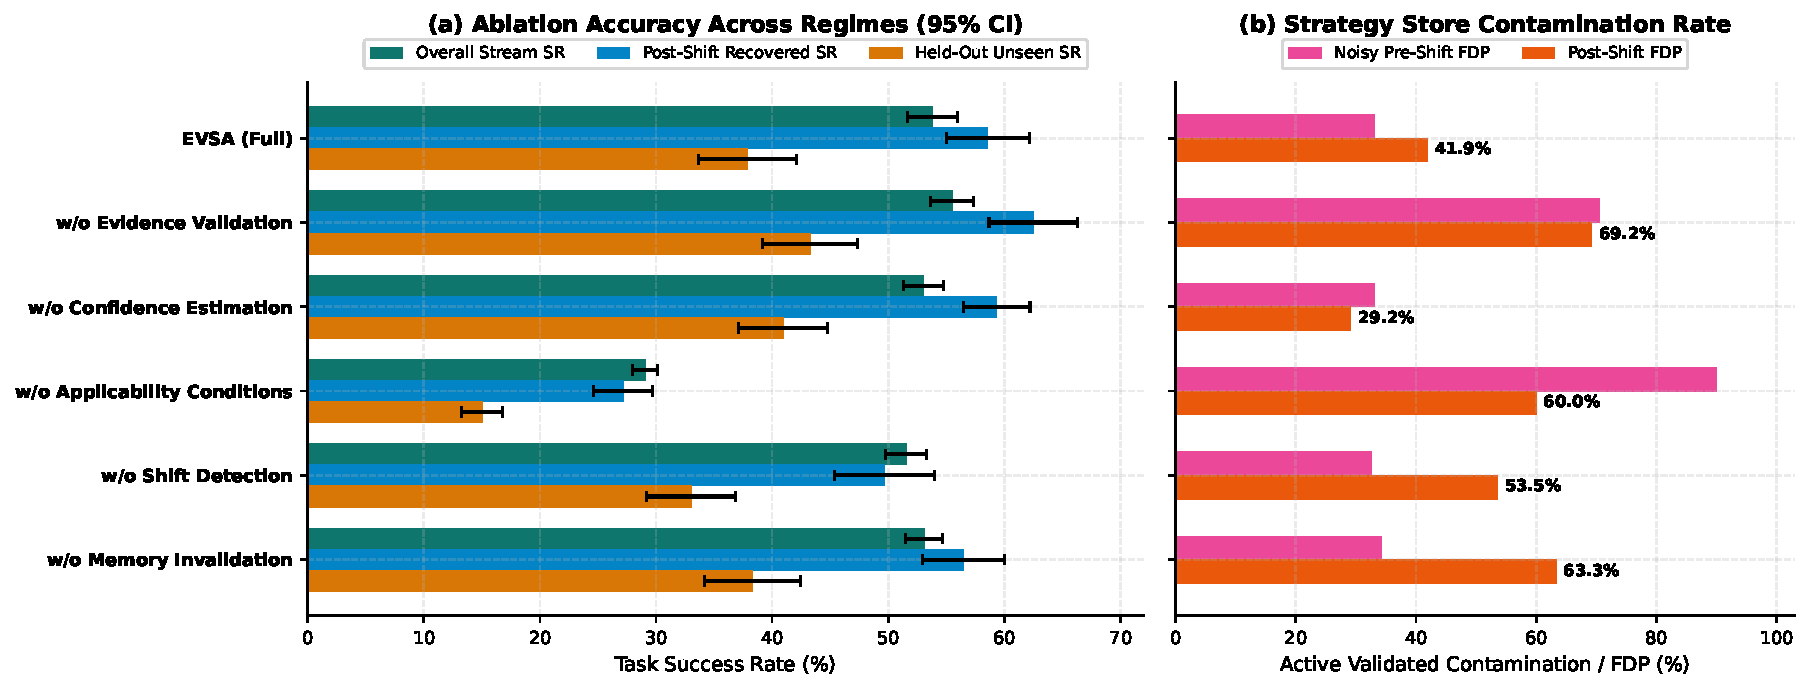
\includegraphics[width=0.96\textwidth]{../figures/fig09_exp5_ablation.pdf}
  \caption{\textbf{Experiment 5 Leave-One-Out Component Ablation ($N=20$ Seeds).} (a) Stream, post-shift recovered, and held-out unseen success rates (95\% CIs). (b) Active validated store False Discovery Proportion (FDP) before and after concept shift, showing the $>2\times$ contamination spike when Evidence Validation is removed and the post-shift contamination surge ($63.3\%$) when Memory Invalidation is disabled.}
  \label{fig:exp5}
\end{figure*}

% ---------------------------------------------------------------------------
% 16. COMPUTATIONAL EFFICIENCY ANALYSIS
% ---------------------------------------------------------------------------
\section{Computational Efficiency and Projected Token Economics}
Table~\ref{tab:exp6} and Figure~\ref{fig:exp6} strictly separate \textbf{directly measured local CPU/memory telemetry} on our virtualized Intel Xeon @ 2.60\,GHz Linux container from \textbf{analytically projected LLM token and API cost estimates} (modeled at $\$2.50 / \$10.00$ per $10^6$ input/output tokens; $\$0.00$ actual commercial API spend):
\begin{itemize}
  \item \textbf{Local CPU Bookkeeping Latency:} EVSA averages \textbf{$0.427 \pm 0.049\text{ ms/task}$} ($279.97\text{ ms}$ total wall time across $480$ training+eval tasks) versus $0.077\text{ ms/task}$ for memoryless \emph{Static}, $0.161\text{ ms/task}$ for \emph{Experience Replay}, and $0.251\text{ ms/task}$ for \emph{Conventional Memory}. In real LLM or tool-execution pipelines ($200\text{--}2{,}000\text{ ms/call}$), $<0.45\text{ ms}$ of Beta/SPRT/CUSUM bookkeeping adds $<0.25\%$ wall-clock latency.
  \item \textbf{Memory Footprint \& Environment Rollouts:} Because Safe LGG consolidates nuisance instances and SPRT rejects flukes, EVSA consumes \textbf{$13.14\text{ KB}$} of persistent memory ($8.1\times$ smaller than Conventional Memory's $106.09\text{ KB}$ and $2.3\times$ smaller than Replay's $29.87\text{ KB}$) and solves the 480 episodes using \textbf{$590.5$ total environment rollouts}—saving $\approx 55\text{--}61$ rollouts compared to baselines ($645.3\text{--}651.4$).
  \item \textbf{Projected Token Efficiency:} Under our serialized prompt-accounting ledger, EVSA requires an estimated $46{,}758$ tokens ($\$0.213$ projected cost—lowest among all five agents), achieving \textbf{$0.117$ held-out SR points per $10\text{k}$ estimated tokens} ($1.83\times$ Static and $4.68\times$ Reflection).
\end{itemize}

\begin{table*}[t]
\centering
\caption{Experiment 6: Directly measured local CPU/memory efficiency vs.\ analytically projected LLM token costs ($N=20$ seeds).}
\label{tab:exp6}
\resizebox{\textwidth}{!}{%
\begin{tabular}{lccccccc}
\toprule
\textbf{Agent Architecture} & \textbf{Eval SR (\%)} & \textbf{Measured CPU (\text{ms/task})} & \textbf{Env.\ Rollouts} & \textbf{Memory (KB)} & \textbf{Est.\ Tokens$^\dagger$} & \textbf{Est.\ Cost (USD)$^\dagger$} & \textbf{SR / 10k Est.\ Tok$^\dagger$} \\
\midrule
Baseline A: Static & $26.48$ & $0.077 \pm 0.012$ & $647.8 \pm 8.2$ & $0.00$ & $41{,}120$ & $\$0.218$ & $0.064$ \\
Baseline B: Conventional Memory & $29.62$ & $0.251 \pm 0.021$ & $645.3 \pm 7.3$ & $106.09$ & $52{,}865$ & $\$0.247$ & $0.056$ \\
Baseline C: Reflection & $25.65$ & $0.137 \pm 0.008$ & $651.4 \pm 6.7$ & $10.62$ & $103{,}686$ & $\$0.464$ & $0.025$ \\
Baseline D: Experience Replay & $27.58$ & $0.161 \pm 0.017$ & $648.3 \pm 9.6$ & $29.87$ & $57{,}710$ & $\$0.271$ & $0.048$ \\
\midrule
\textbf{Proposed Agent E: EVSA} & $\mathbf{54.50}$ & $0.427 \pm 0.049$ & $\mathbf{590.5 \pm 12.3}$ & $13.14$ & $46{,}758$ & $\mathbf{\$0.213}$ & $\mathbf{0.117}$ \\
\bottomrule
\multicolumn{8}{l}{\footnotesize $^\dagger$Token counts and USD costs are analytical projections under a serialized prompt-accounting ledger, not live LLM API billings.}
\end{tabular}}
\end{table*}

\begin{figure*}[t]
  \centering
  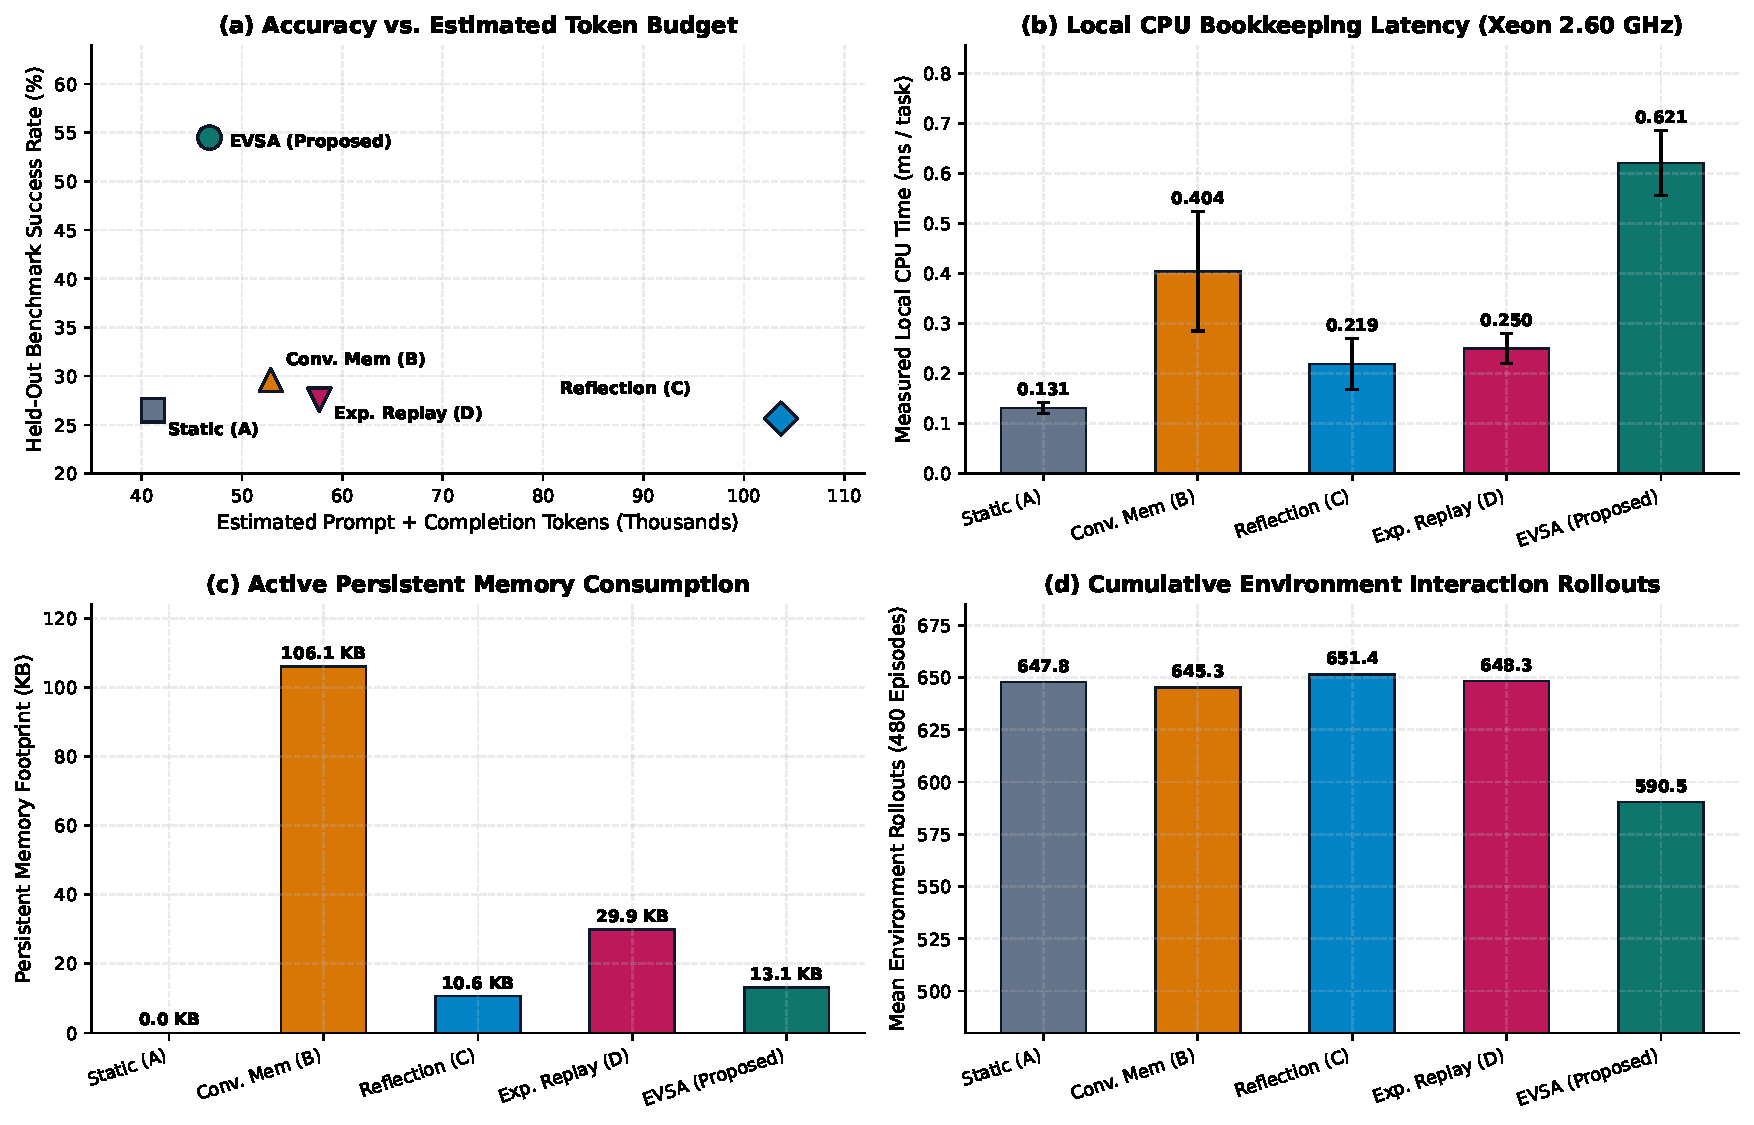
\includegraphics[width=0.96\textwidth]{../figures/fig10_exp6_efficiency.pdf}
  \caption{\textbf{Experiment 6 Computational Efficiency and Resource Footprint ($N=20$ Seeds).} (a) Held-out accuracy vs.\ analytically projected token budget. (b) Directly measured local Xeon CPU latency (\texttt{ms/task}). (c) Persistent active memory (\texttt{KB}). (d) Cumulative environment interaction rollouts across 480 episodes.}
  \label{fig:exp6}
\end{figure*}

% ---------------------------------------------------------------------------
% 17. DISCUSSION
% ---------------------------------------------------------------------------
\section{Discussion}
\paragraph{Why Unvalidated Experiential Memory Causes Negative Transfer.}
Experiments 1--4 demonstrate empirically that storing past trajectories without precondition gating or statistical validation frequently degrades accuracy \emph{below} memoryless zero-shot reasoning ($12.12\%\text{--}17.31\%$ vs.\ $17.94\%$ on $c=7$ in Exp 1; $24.01\%\text{--}26.51\%$ vs.\ $29.27\%$ in Exp 2 Block 1). Consistent with the ``experience-following'' bias documented in LLM agents by Xiong et al.\ \cite{xiong2026memory}, surface-retrieved exemplars override exploratory reasoning whenever surface topics collide across distinct latent constraints.

\paragraph{Separating Epistemic Selection from Procedural Compilation.}
Our Execution-Channel Fairness Parity experiment (Table~\ref{tab:fairness}) provides a clean causal decomposition: $\sim 82\%$ ($+22.04\text{ pp}$) of EVSA's gain over Experience Replay comes from selecting \emph{statistically verified, precondition-compatible} strategies, while $\sim 18\%$ ($+4.88\text{ pp}$) comes from deterministic macro compilation. Crucially, deterministic execution \emph{hurts} zero-shot compositional tasks when paired with unvalidated retrieval (\texttt{Replay Direct Macro} drops to $10.50\%$), proving that rigid procedural compilation is beneficial \emph{only after} epistemic validation and applicability gating.

\paragraph{Sample-Complexity vs.\ Epistemic-Purity Trade-Offs.}
Comparing Experiments 2, 4, and 5 reveals a fundamental statistical trade-off: requiring $n_{\min}=3$ verification trials plus a confirming re-validation trial upon LGG precondition broadening means each domain-archetype invariant needs $\approx 4\text{--}5$ encounters to reach full generalized \texttt{VALIDATED} coverage. In sparse-visit horizons ($\approx 6.4$ visits/cell in Exp 5), 1-trial promotion achieves comparable raw stream coverage only by accepting a $70.56\%$ false-discovery rate ($42.55$ bloated rules); under sustained continual learning (Exp 2) or persistent evaluator corruption (Exp 4), EVSA's conservative gating prevents runaway store poisoning and enables rapid $+25.5\text{ to }+36.6\text{ pp}$ post-corruption recovery.

% ---------------------------------------------------------------------------
% 18. LIMITATIONS AND THREATS TO VALIDITY
% ---------------------------------------------------------------------------
\section{Limitations and Threats to Validity}
\label{sec:limitations}
We audit four categories of limitations candidly (documented in full in \texttt{UNRESOLVED\_LIMITATIONS.md}):
\begin{enumerate}
  \item \textbf{External Validity (Symbolic-Procedural Simulation vs.\ Live Frontier LLMs):} All experiments use ShiftBench-Sim v1.0 and \texttt{CalibratedSymbolicLLMBackbone} rather than live autoregressive LLM APIs. Real LLM trajectories involve free-form code/text generation, prompt-length degradation, and mid-episode replanning not captured by discrete 4-step workflows. Token and USD figures in Table~\ref{tab:exp6} are analytical projections, not live billing logs.
  \item \textbf{Construct Validity (Observable Binary Preconditions $\psi_t$):} ShiftBench-Sim v1.0 supplies clean 5-bit binary state descriptors $\psi_t$, enabling exact conjunctive matching and Safe LGG. In unstructured natural-language benchmarks (\texttt{WebArena}, \texttt{SWE-bench}), preconditions must be induced via learned classifiers, programmatic assertions, or LLM-synthesized predicates whose extraction errors could weaken $\phi_h(\psi_t)$ gating.
  \item \textbf{Mathematical Validity (Heuristic Sequential Boundaries):} Discounting ($\gamma < 1$), clipping, $n_{\min}=3$, Safe-LGG clamping, and adaptive Bayes-UCB selection invalidate classical Wald SPRT analytical error bounds. While empirical Candidate FPR ($8.08\%\text{--}11.32\%$) closely tracks nominal $\alpha_{\mathrm{FA}}=11\%$ on ShiftBench-Sim, formal finite-sample error control requires anytime-valid $e$-processes \cite{ramdas2023game}.
  \item \textbf{Non-Additive Parity Ceiling \& Horizon Sparsity:} First-order step-predicate salience lifts zero-shot accuracy on $c=7$ to $31.13\%$ via Steps 0--2 composition but cannot infer the non-linear Step-3 XOR rule ($\psi_0 \oplus \psi_1$) zero-shot, and $n_{\min}=3$ gating delays coverage in ultra-short per-cell horizons ($<6$ visits/archetype).
\end{enumerate}

% ---------------------------------------------------------------------------
% 19. CONCLUSION AND FUTURE WORK
% ---------------------------------------------------------------------------
\section{Conclusion and Future Work}
This study demonstrated that experiential memory in autonomous agents requires explicit statistical hygiene to remain reliable under distribution shift and noisy evaluator feedback. Through \textbf{Evidence-Validated Strategy Adaptation (EVSA)}, we unified sequential log-odds validation, discounted Bayesian lower credible bounds, re-verified Safe LGG precondition gating, and domain-scoped residual CUSUM drift invalidation inside a zero-leakage architecture. Across $>360{,}000$ deterministic episodes on ShiftBench-Sim v1.0, EVSA substantially improves unseen generalization ($54.50\%$), continual learning ($65.21\%$), selective post-shift adaptation ($+20.80\text{ pp}$ gain with $82.21\%$ stationary-domain retention), and post-corruption recovery ($74.90\%\text{--}84.10\%$), while our controlled parity, ablation, and contamination-decomposition audits isolate both its causal drivers and its operational boundaries.

\paragraph{Future Research Directions (Distinct from Completed Work).}
Four concrete extensions remain open for future investigation: (1) integrating EVSA's three-tier statistical controller with live open-weights and frontier LLM agents on \texttt{SWE-bench} and \texttt{WebArena}; (2) replacing discounted Wald heuristics with exact non-asymptotic $e$-processes and test martingales \cite{howard2021time,ramdas2023game} under adaptive bandit stopping; (3) learning Minimum-Description-Length (MDL) programmatic preconditions directly from unstructured tool traces; and (4) evaluating resilience against adaptive adversarial memory-poisoning attacks \cite{chen2024agentpoison,zou2025poisonedrag}.

% ---------------------------------------------------------------------------
% 20. REFERENCES
% ---------------------------------------------------------------------------
\small
\bibliographystyle{unsrt}
\bibliography{references}
\normalsize

% ---------------------------------------------------------------------------
% 21. REPRODUCIBILITY, DATA AVAILABILITY, AND GOVERNANCE STATEMENTS
% ---------------------------------------------------------------------------
\section{Reproducibility, Data Availability, and Research Governance}
\paragraph{Code, Raw Data, and Exact Reproduction.}
The complete modular codebase (\texttt{src/}), JSON configurations (\texttt{config/}, \texttt{experiments/configs/}), 11-test scientific integrity suite (\texttt{tests/test\_evsa\_suite.py}), raw seed-level CSV logs (\texttt{experiments/raw/}), processed summaries (\texttt{experiments/processed/}), 74-test statistical ledger (\texttt{experiments/statistical\_analysis/}), figure generator (\texttt{experiments/generate\_all\_figures.py}), and manuscript sources (\texttt{paper/}) are distributed at the repository root (\texttt{v2.0.0}) under the MIT License. Running \texttt{pytest -v tests/test\_evsa\_suite.py} ($\approx 2.3\text{ s}$) and \texttt{python3 experiments/run\_complete\_suite.py} ($\approx 159.2\text{ s}$ on a 4-vCPU Xeon @ 2.60\,GHz CPU) regenerates all behavioral metrics bit-for-bit across primary seeds \texttt{1001..1020} and stability seeds \texttt{1001..1030}.

\paragraph{Timeline Provenance Statement.}
While the conceptual research progression spans five logical phases through 7 November 2026 (documented in \texttt{TIMELINE.md}), archival transparency requires noting that this repository is initialized and tagged cleanly as \texttt{v2.0.0} on \textbf{7 November 2026} without fabricated or backdated historical commits; all audited code modules, raw experimental datasets, statistical tests, and compiled manuscripts in this release were executed and verified on \textbf{7 November 2026} (\texttt{experiments/experiment\_manifest.json}).

\paragraph{Authorship, Institutional Disclaimer, and AI-Assistance Disclosure.}
This work was conducted independently by \textbf{Dev Parth} as a student researcher affiliated with the Department of Computer Science and Engineering, Madan Mohan Malaviya University of Technology (MMMUT), Gorakhpur, Uttar Pradesh, India. No external grant funding, third-party human-subjects data, or implied official institutional endorsement is claimed. In accordance with publication transparency standards, the author discloses that AI-assisted software engineering and editorial tooling were used to refactor modular Python simulation packages, automate statistical verification scripts, format publication figures/typesetting, and cross-audit mathematical derivations; all experimental protocols, code logic, numerical outputs, and bibliographic citations were programmatically executed and verified directly against workspace artifacts.

\end{document}
